\chapter{免疫应答}
\begin{framed}
\noindent\textbf{【知识体系】}
\begin{center}
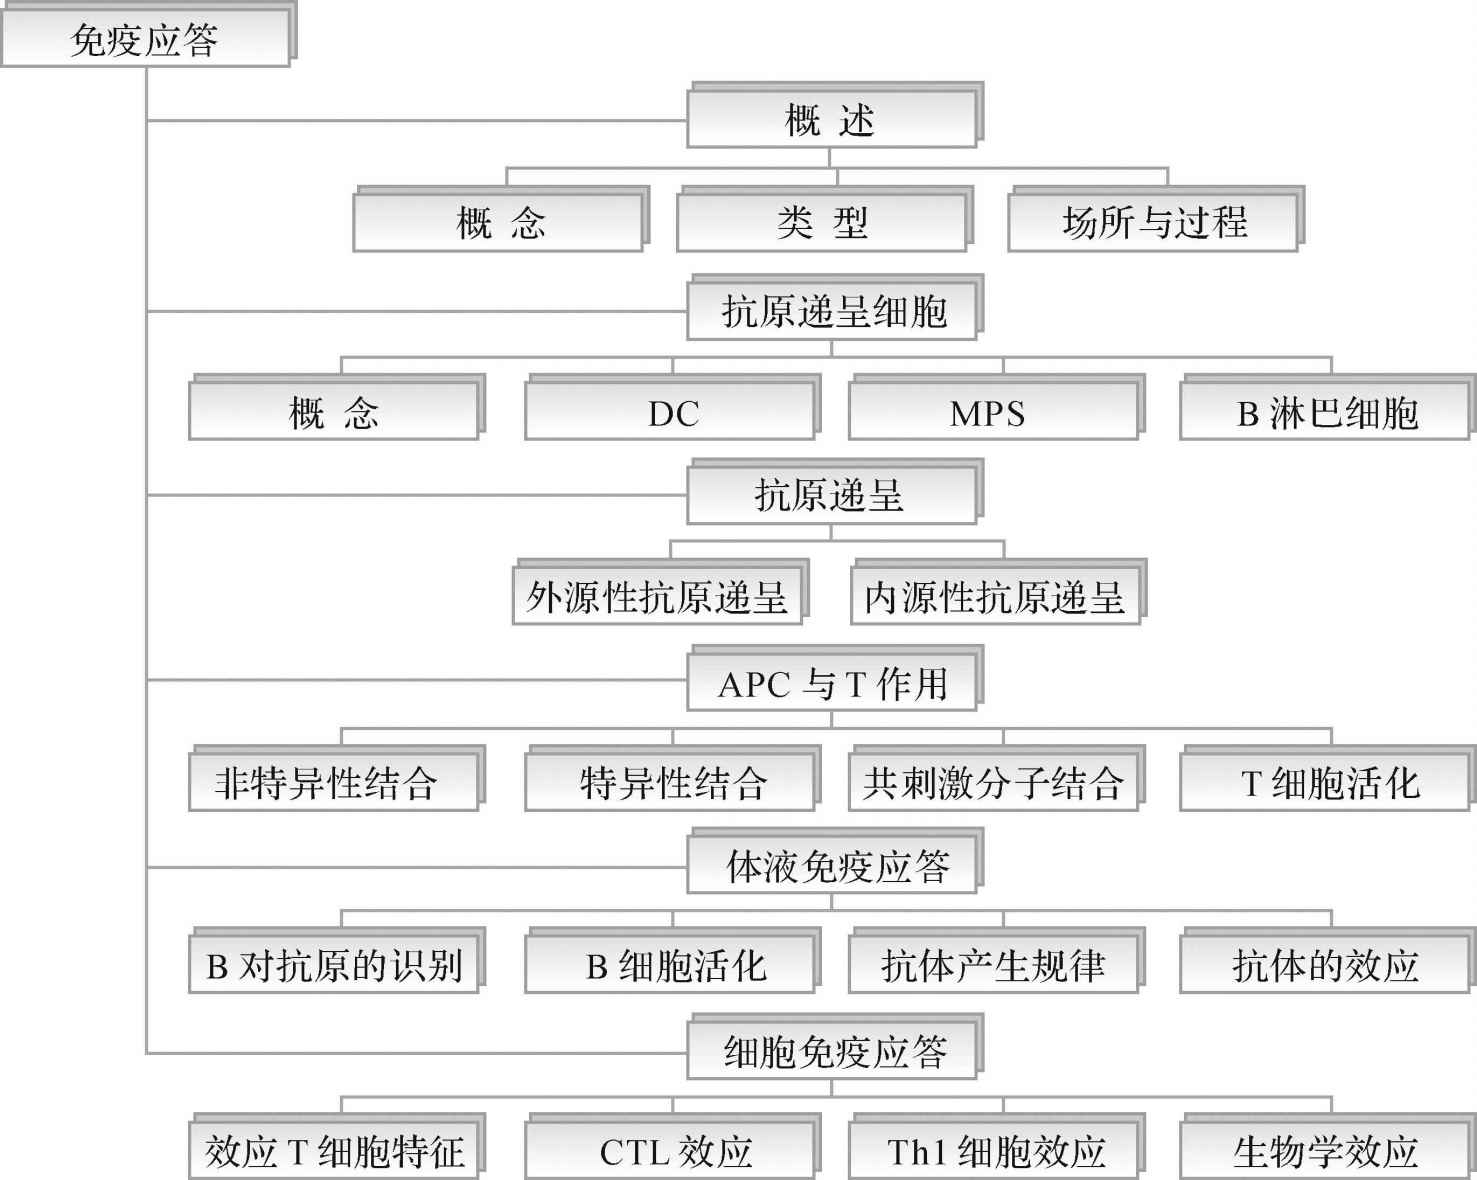
\includegraphics{./images/Image00126.jpg}
\end{center}
\noindent\textbf{【课前思考】}

当病原体入侵或体内细胞癌变时,机体产生什么样的反应?机体是通过什么反应排除异物达到体内内环境稳定的?整个应答过程如何?针对不同抗原,机体是如何产生不同应答的?体内抗体的产生有什么规律?

\noindent\textbf{【本章重点】}

1.免疫应答的概念、类型、应答场所、过程;

2.T、B细胞介导的免疫应答过程、特点、效应;

3.抗体产生的规律及应用。

\noindent\textbf{【教学目标】}

1.熟悉单核吞噬细胞系统、树突状细胞、B细胞生物学特性、递呈抗原的基本特点;

2.掌握免疫应答的概念、类型、应答场所、过程;

3.掌握抗体产生的一般规律;

4.熟悉T、B细胞介导的免疫应答过程、特点、效应。
\end{framed}

\section{概述}


\subsection{概念}

免疫应答是指机体受抗原性异物刺激后,体内免疫细胞发生一系列反应以排除抗原性异物的生理过程。免疫应答最基本的生物学意义是识别“自己”与“非己”,从而清除“非己”的抗原性物质,保护机体免受异己抗原的侵袭。

免疫应答主要包括:(1)APC对Ag的加工、处理、递呈;(2)淋巴细胞识别Ag后,自身活化、增殖、分化产生免疫效应。

其生物学意义:及时清除体内抗原性异物,以保持内环境的恒定。但在某些情况下,免疫应答也会对机体造成损伤,如超敏反应。


\subsection{类型}

根据参与免疫应答和介导免疫效应的组分和细胞种类的不同,特异性免疫应答还可分为B细胞介导的体液免疫(humoral
immunity)和T细胞介导的细胞免疫(cellular immunity)。

在某些特定条件下,抗原也能诱导机体免疫系统对其产生特异性不应答状态------免疫耐受性或称负免疫应答。


\subsection{免疫应答场所与过程}

特异性免疫应答发生的场所主要在外周免疫器官(淋巴结和脾脏)。整个应答过程分为三个阶段:①感应阶段(Ag识别阶段):包括抗原的摄取、处理、递呈和特异性识别;②反应阶段(增生分化阶段):指免疫细胞(T、B细胞)识别抗原后传递活化信号,自身发生活化、增殖和分化;③效应阶段:引发T细胞介导的细胞免疫效应和B细胞介导的体液免疫效应。

\section{抗原递呈细胞}

抗原递呈细胞(antigen-presenting
cell,APC)是能摄取、加工处理抗原,并将抗原递呈给淋巴细胞的一类免疫细胞,在机体免疫应答过程中发挥重要作用(图\ref{fig9-1})。此类细胞能辅助和调节T细胞、B细胞识别抗原并对抗原产生应答,故又称为辅佐细胞(accessory
cell),简称A细胞。根据APC细胞表面膜分子表达情况和功能的差异,可将其分为:

专职(professiona)
APC:能表达MHC-Ⅱ类抗原和其他参与T细胞活化的共刺激分子,包括单核吞噬细胞系统(mononuclear
phagocyte system,MPS)、树突状细胞、B细胞等。

非专职APC:包括内皮细胞、纤维母细胞、上皮细胞等。它们通常情况下并不表达MHC-Ⅱ类分子,但在炎症过程中或受到IFN-γ诱导,也可表达MHC-Ⅱ类分子并处理和递呈抗原。

另外,机体有核细胞能将内源性蛋白抗原降解处理为多肽片段,后者与I类分子结合为复合物表达在细胞表面,并递呈给CD8\textsuperscript{+}
TC细胞。以前曾不将此类细胞归于严格意义上的APC,而是称其为靶细胞,但近年亦将其称为APC。目前对APC的定义为:所有表达MHC分子并能处理和递呈抗原的细胞。

\begin{figure}[!htbp]
 \centering
 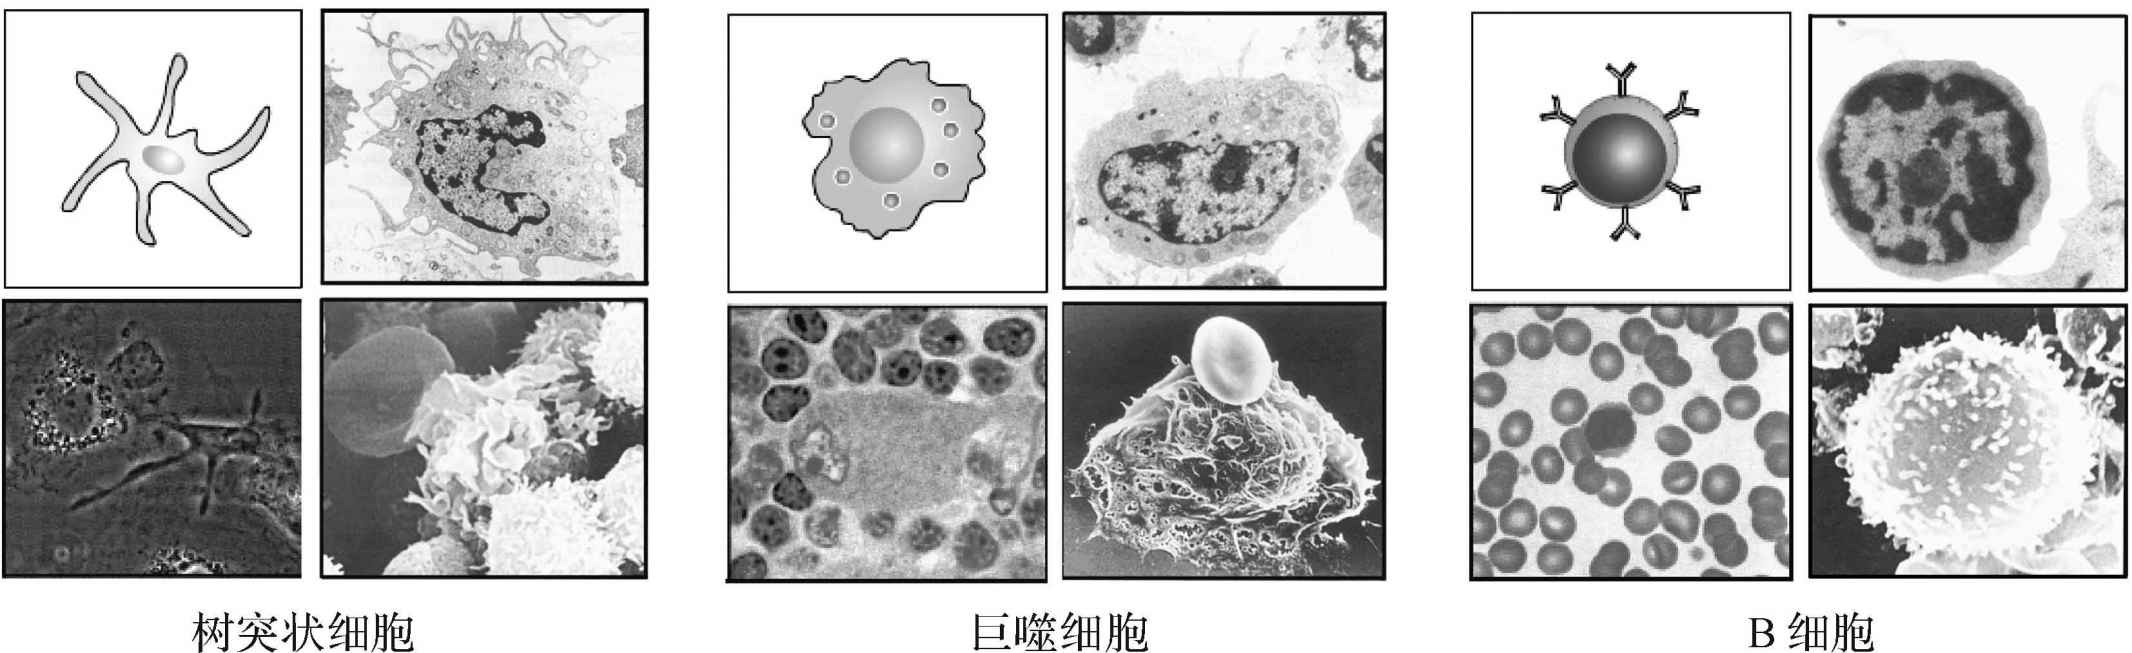
\includegraphics[width=.7\textwidth]{./images/Image00127.jpg}
 \captionsetup{justification=centering}
 \caption{抗原递呈细胞}
 \label{fig9-1}
  \end{figure} 


\subsection{基本概念}

抗原加工:蛋白质抗原在细胞内被降解成能与MHC分子结合的肽的过程。

抗原递呈:MHC分子与抗原肽结合,将其展示于细胞表面供T细胞识别的过程(图\ref{fig9-2})。

\begin{figure}[!htbp]
 \centering
 
\includegraphics{./images/Image00128.jpg}
 \captionsetup{justification=centering}
 \caption{抗原递呈示意图}
 \label{fig9-2}
  \end{figure} 

内源性抗原:细胞内产生的蛋白质抗原,包括自身抗原和非己抗原------MHC-Ⅰ类分子递呈。

外源性抗原:由细胞外摄入细胞内的蛋白质抗原,包括非己抗原和自身抗原------MHC-Ⅱ类分子递呈。


\subsection{树突状细胞(dendritic cell,DC)}

树突状细胞是由美国学者Steinman于1973年所发现,因其成熟细胞具有许多树突样或伪足样突起而得名。DC是目前所知体内功能最强的专职APC,与其他APC相比,其最大特点是能够刺激初始T细胞(naive
T
cell)增殖,而MM、B细胞则仅能刺激已活化的或记忆性T细胞,故DC是机体免疫应答的启动者,在免疫系统中占有独特的地位。对DC的研究不仅有助于阐明机体免疫应答的调控机理,也对认识肿瘤、移植排斥反应、感染、自身免疫病的发生机制并制订有效的防治措施具有重要意义。

(一) DC的来源、分化和种类

DC主要由骨髓中髓样干细胞分化而来,与单核吞噬细胞有共同的前体细胞,这些髓系来源的DC称为髓样DC(myeloid
DC,MDC)。部分DC由淋巴样干细胞分化而来,与淋巴细胞有共同的前体细胞,此类淋巴系来源的DC称为淋巴样DC(lymphoid
DC,LDC)(图\ref{fig9-3})。

\begin{figure}[!htbp]
 \centering
 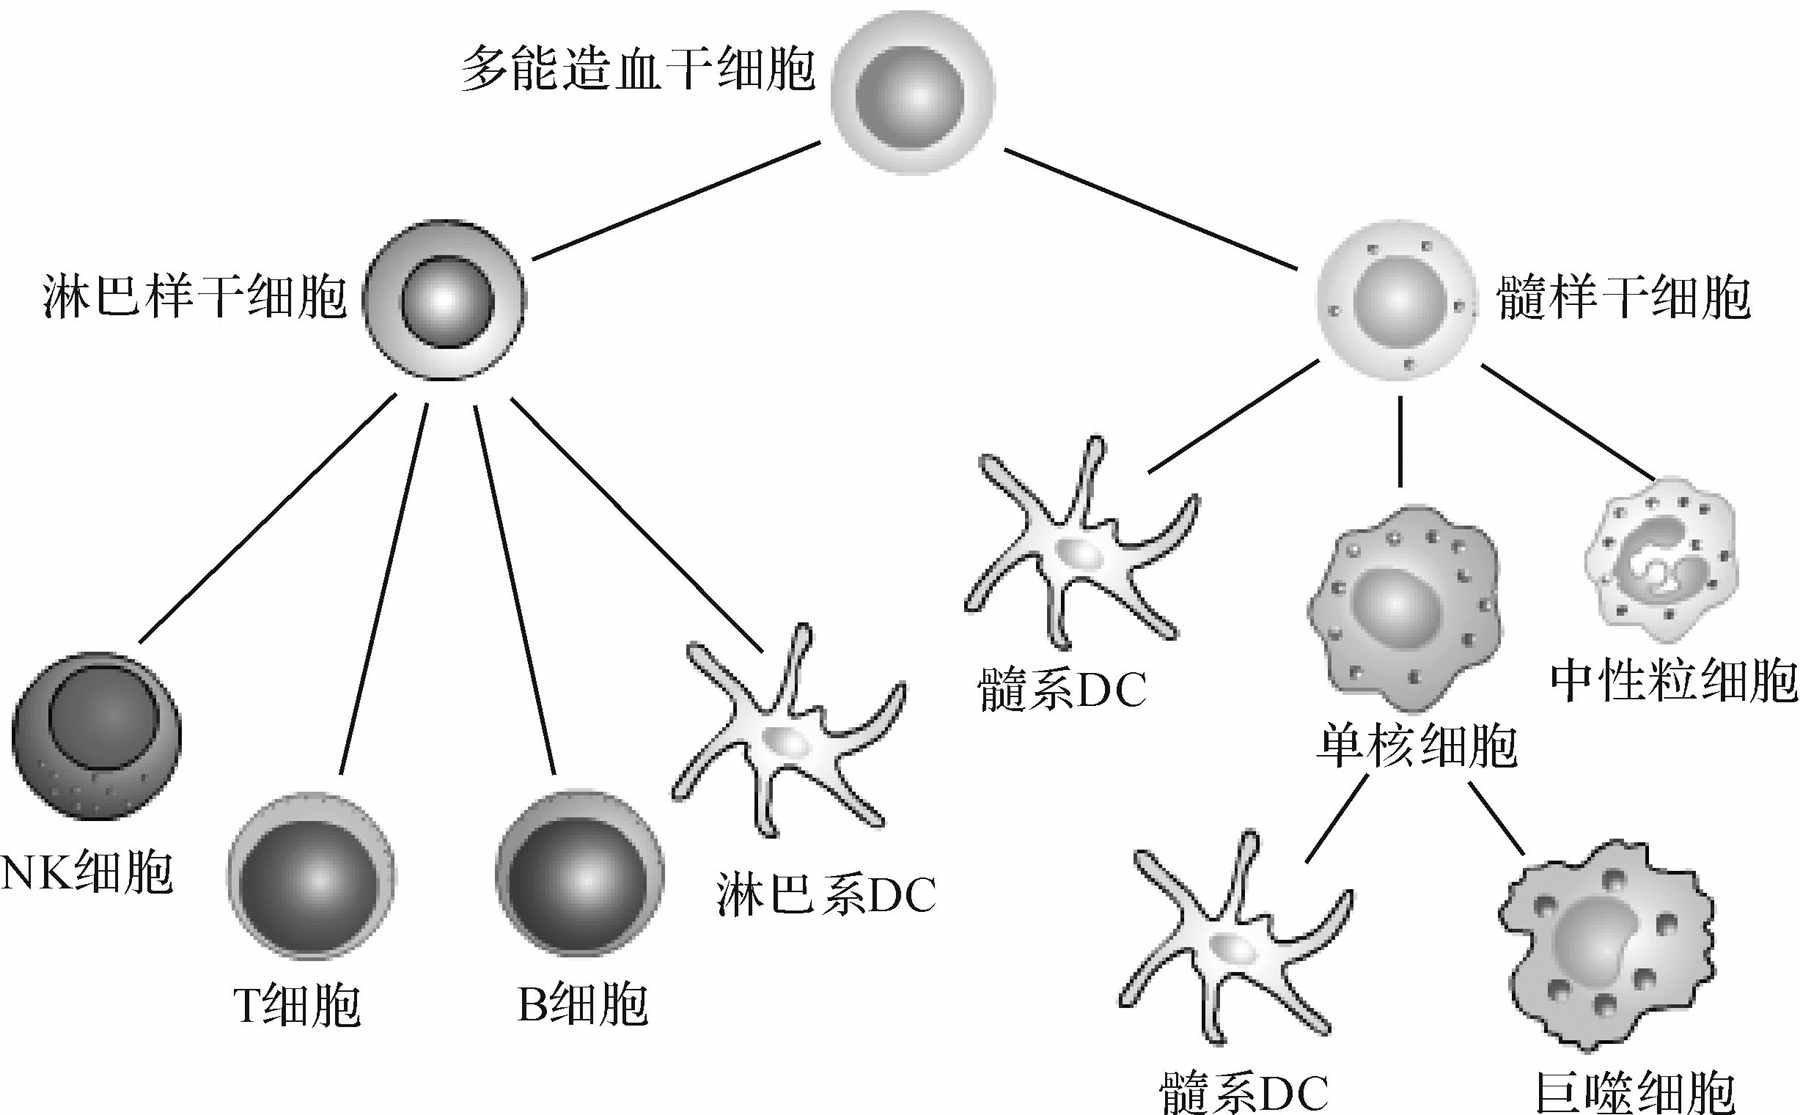
\includegraphics{./images/Image00129.jpg}
 \captionsetup{justification=centering}
 \caption{树突状细胞的来源}
 \label{fig9-3}
  \end{figure} 

DC广泛分布于(脑以外)全身各组织和器官,但数量极少,分布在不同部位和处于不同分化阶段的DC具有不同的生物学特征和命名,主要有:

(1)郎格罕斯细胞(Langerhans
cell,LC):LC是位于表皮和胃肠道上皮部位的未成熟DC,其高表达FcgR、C3bR、MHC-I/II类分子,胞浆内含特征性Birbeck颗粒。

(2)并指状DC(interdigitating
DC,IDC):IDC存在于外周淋巴组织的胸腺依赖区,是由LC或间质性DC移行至淋巴结而衍生的成熟DC,其表面缺乏FcR及C3bR,但高表达MHC-I、-II类分子和B7,通过其突起与T细胞密切接触,将抗原递呈给T细胞,具有较强的免疫激发作用。

(二)生物学功能

DC是体内最重要的APC,并具有其他生物学功能。

1.抗原递呈功能。

2.调节免疫应答:DC能递呈抗原并激发免疫应答,尤其是能激活初始T细胞,此效应是启动特异性免疫应答的关键步骤,如图\ref{fig9-4}所示。

\begin{figure}[!htbp]
 \centering
 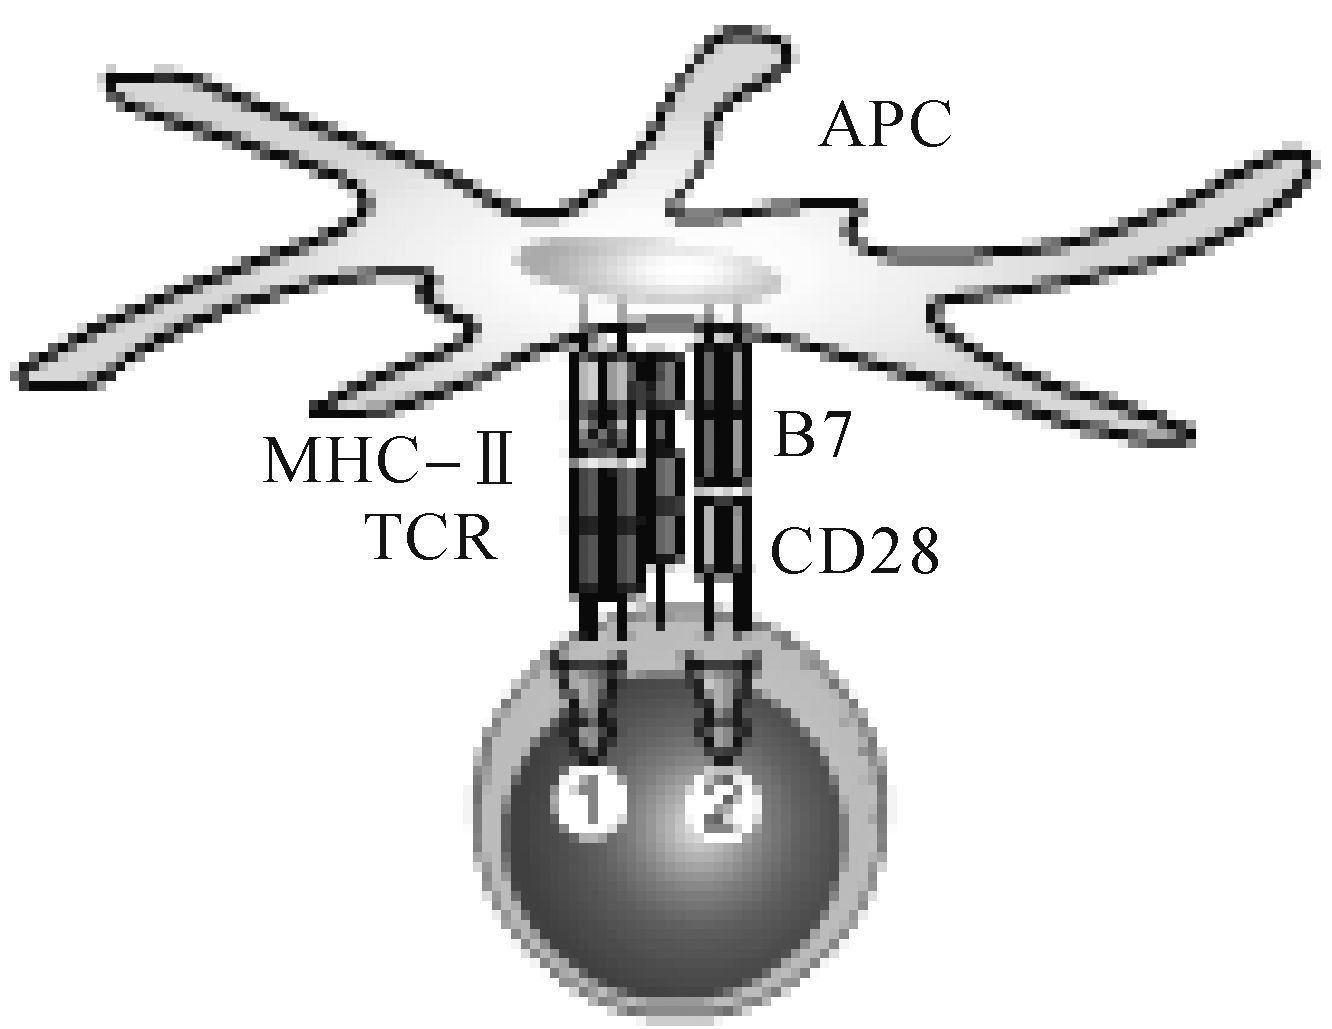
\includegraphics{./images/Image00130.jpg}
 \captionsetup{justification=centering}
 \caption{DC能递呈抗原并激发免疫应答}
 \label{fig9-4}
  \end{figure} 


\subsection{单核吞噬细胞系统(mononuclear phagovyte system,MPS)}

单核吞噬细胞系统包括骨髓中的前单核细胞(pre-monocyte)、外周血中的单核细胞(monocyte,Mon)以及组织内的巨噬细胞(macrophage,Mφ),是体内具有最活跃生物学功能的细胞类型之一。

(一)生物活性成分

单核吞噬细胞能产生各种溶酶体酶、溶菌酶、髓过氧化物酶等。Mφ(尤其是活化的Mφ)还能产生和分泌近百种生物活性物质,如细胞因子(IL-1、IL-6、IL-12等)、补体成分(C1、P因子等)、凝血因子,以及前列腺素、白三烯、血小板活化因子、ACTH、内啡肽等活性产物。随Mφ所受刺激、所处活化阶段和活化程度不同,上述活性分子的产生和分泌各异,并与Mφ功能状态密切相关。

(二)主要生物学作用

单核/巨噬细胞是参与非特异性免疫和特异性免疫的重要细胞,参与吞噬消化、杀伤肿瘤细胞、加工和递呈抗原、调节免疫应答、介导炎症反应,如图\ref{fig9-5}所示。

\begin{figure}[!htbp]
 \centering
 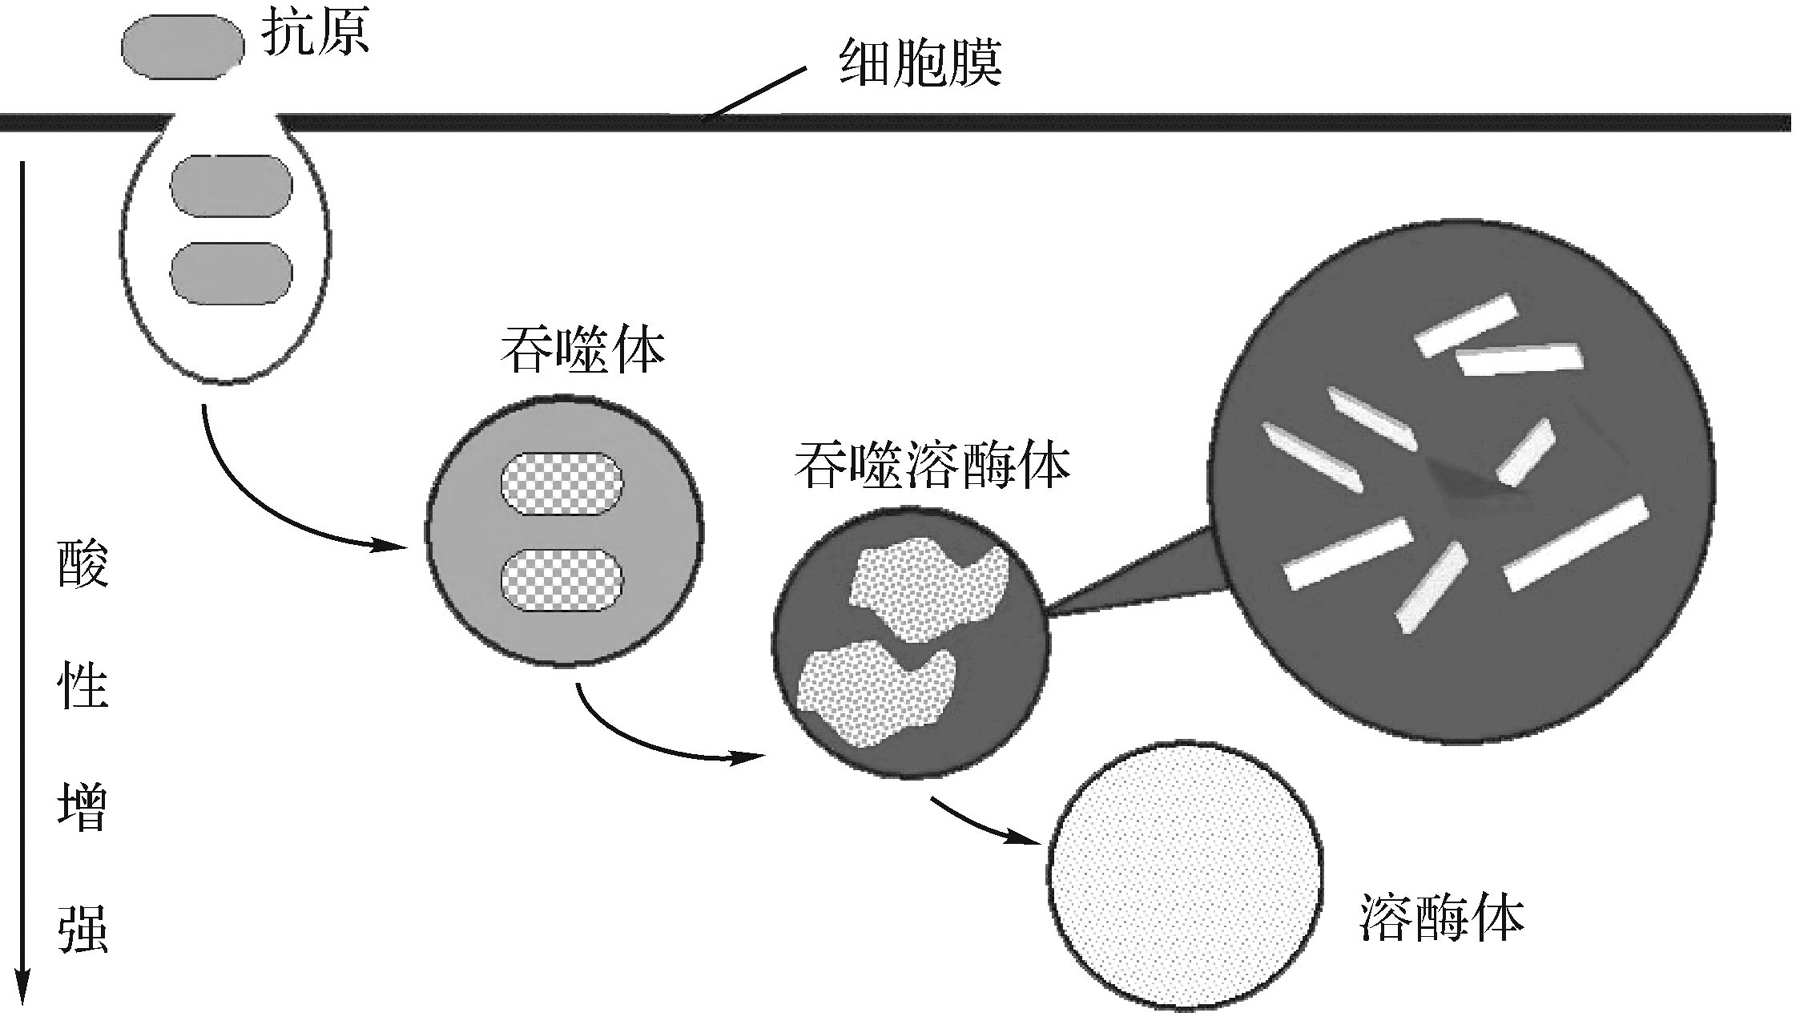
\includegraphics{./images/Image00131.jpg}
 \captionsetup{justification=centering}
 \caption{巨噬细胞的吞噬消化作用}
 \label{fig9-5}
  \end{figure} 


\subsection{B淋巴细胞}

B淋巴细胞是参与体液免疫应答的重要免疫细胞,也是一类重要的专职APC。B细胞高表达MHC-Ⅱ类分子,能摄取、加工处理抗原,并将抗原肽-MHC-Ⅱ类分子复合物表达于细胞表面,递呈给Th细胞,主要通过B细胞表面BCR可特异性识别和结合抗原,再进行内吞。此效应具有浓缩抗原的效应,在抗原浓度非常低的情况下是有效摄入和(向Th
细胞)递呈抗原的方式。另外,BCR在特异性识别和结合抗原的同时,也向B细胞提供了第一活化信号,故此途径对激发针对TD抗原的体液和细胞免疫应答均具有重要意义(图\ref{fig9-6})。

\begin{figure}[!htbp]
 \centering
 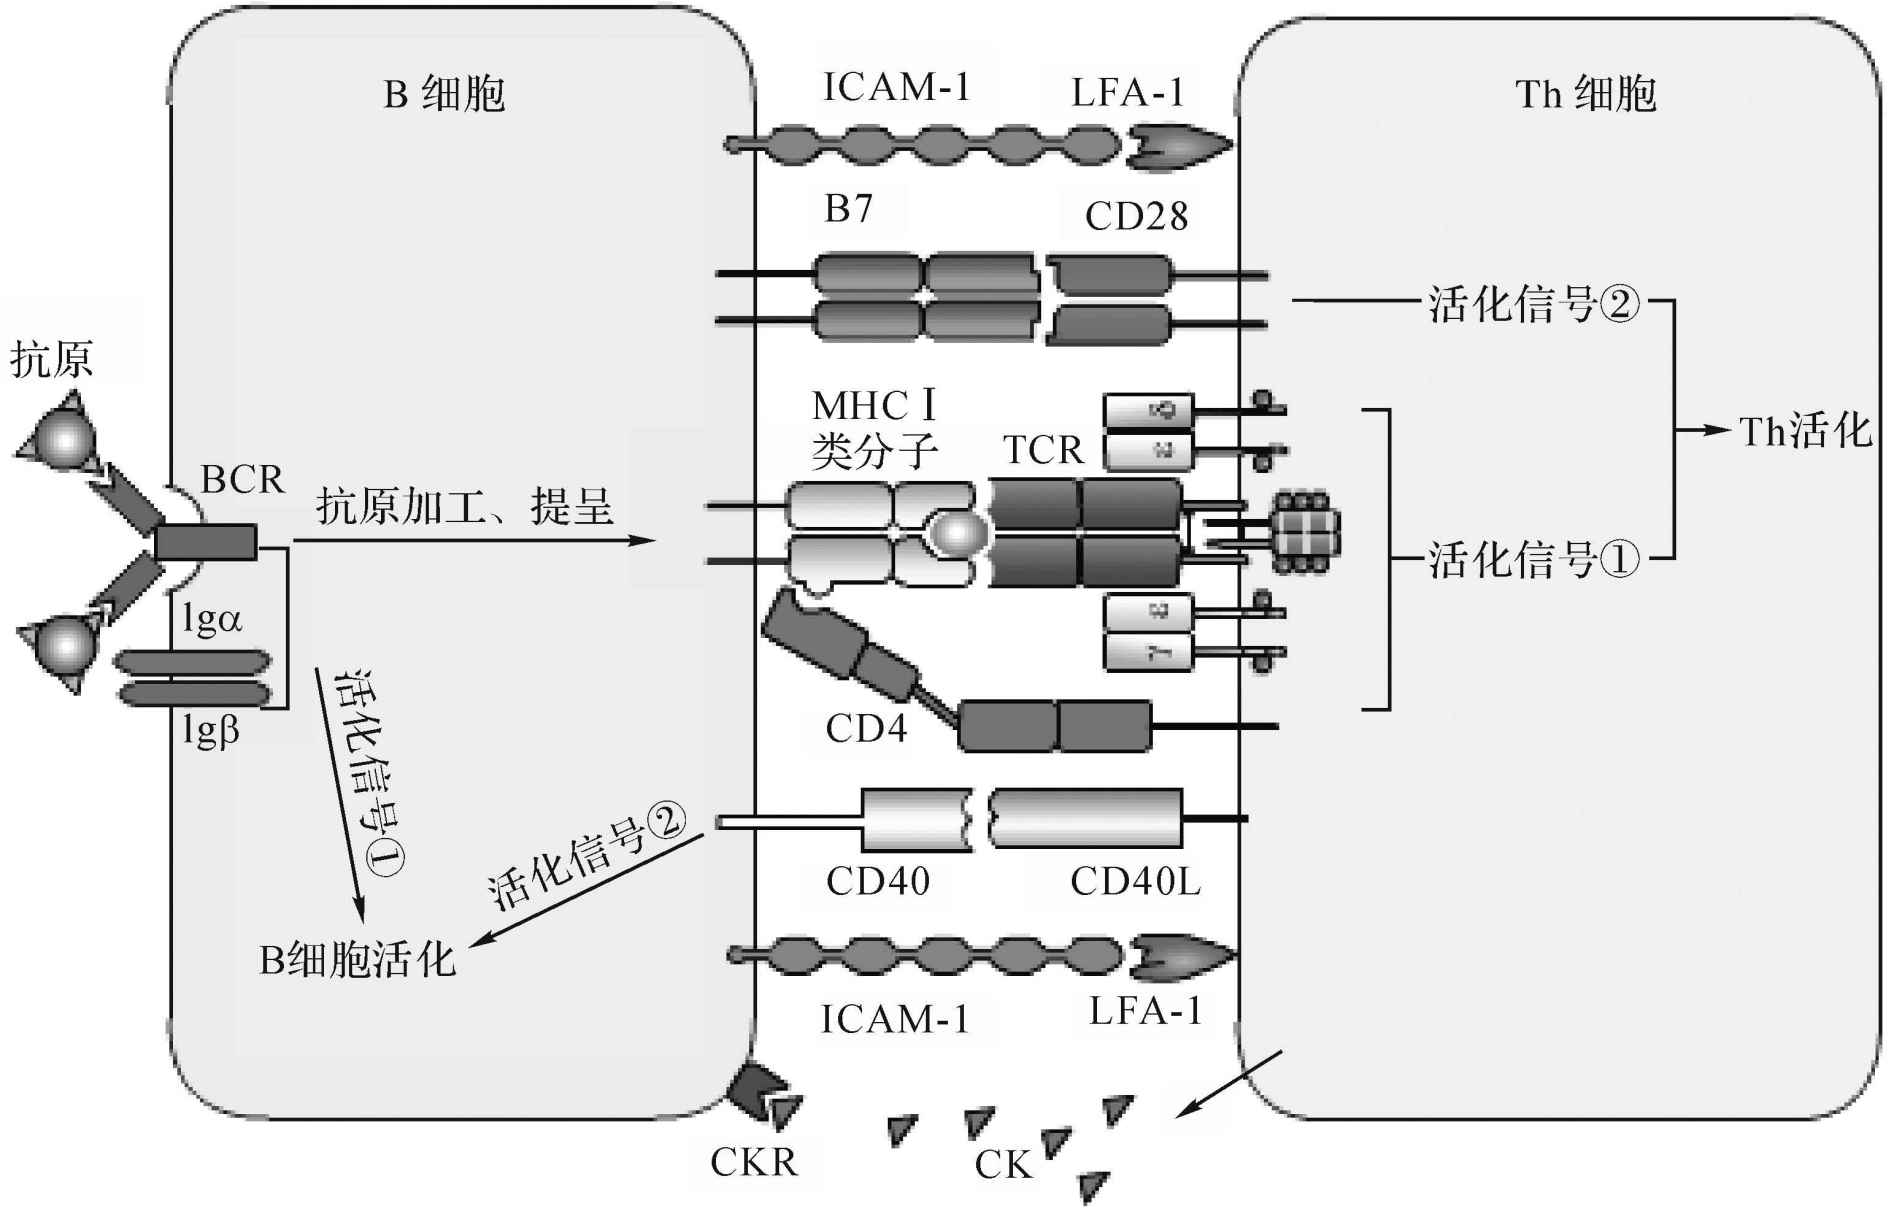
\includegraphics[width=.6\textwidth]{./images/Image00132.jpg}
 \captionsetup{justification=centering}
 \caption{B细胞与Th细胞间的相互作用}
 \label{fig9-6}
  \end{figure} 

\section{抗原递呈}

T细胞借助其表面TCR识别抗原物质,但一般不能直接识别可溶性蛋白抗原,而仅识别与MHC分子结合成复合物的抗原肽:CD4\textsuperscript{+}
T细胞识别APC表面抗原肽-MHC-Ⅱ类分子复合物;CD8\textsuperscript{+}
T细胞识别靶细胞表面抗原肽-MHC-I类分子复合物。细胞将胞浆内自身产生或摄入胞内的抗原消化降解为一定大小的抗原肽片段,以适合与胞内MHC分子结合,此过程称为抗原加工(antigen
processing)或抗原处理。抗原肽与MHC分子结合成抗原肽-MHC分子复合物,并表达在细胞表面,以供T细胞识别,此过程称为抗原递呈(antigen
presenting)。APC或靶细胞对抗原进行加工与递呈,是
TD抗原诱导特异性免疫应答的前提。

根据被递呈抗原的来源不同,可将其分为:

1.外源性抗原(exogenous
antigen):来源于细胞外的抗原,如被吞噬的细胞、细菌或某些自身成分等。APC加工处理外源性抗原后形成的抗原肽,常由MHC-Ⅱ类分子递呈给CD4\textsuperscript{+}
T细胞,此为溶酶体途径或MHC-Ⅱ类途径。

2.内源性抗原(endogenous
antigen):是细胞内合成的抗原,如病毒感染细胞所合成的病毒蛋白、肿瘤细胞合成的蛋白以及胞内某些自身正常成分等。内源性抗原在胞内加工后形成的抗原肽则与MHC-I类分子结合,递呈给CD8\textsuperscript{+}
T细胞,此为胞质溶胶途径或MHC-I类途径。


\subsection{外源性抗原的加工、处理和递呈}

(一)外源性抗原的加工处理

APC通过胞吞作用(endocytosis)或称内化作用(internalization)而摄入外源性抗原,包括吞噬、吞饮或受体介导的内吞作用。所摄入的外源性抗原由胞浆膜包裹,在胞内形成内体(endosome),逐渐向胞浆深处移行,并与溶酶体融合形成内体/溶酶体。内体/溶酶体中含有组织蛋白酶、过氧化氢酶等多种酶,且为酸性环境,可使蛋白抗原降解为含13~18个氨基酸的肽段,适合与MHC-Ⅱ类分子结合(图\ref{fig9-7})。

\begin{figure}[!htbp]
 \centering
 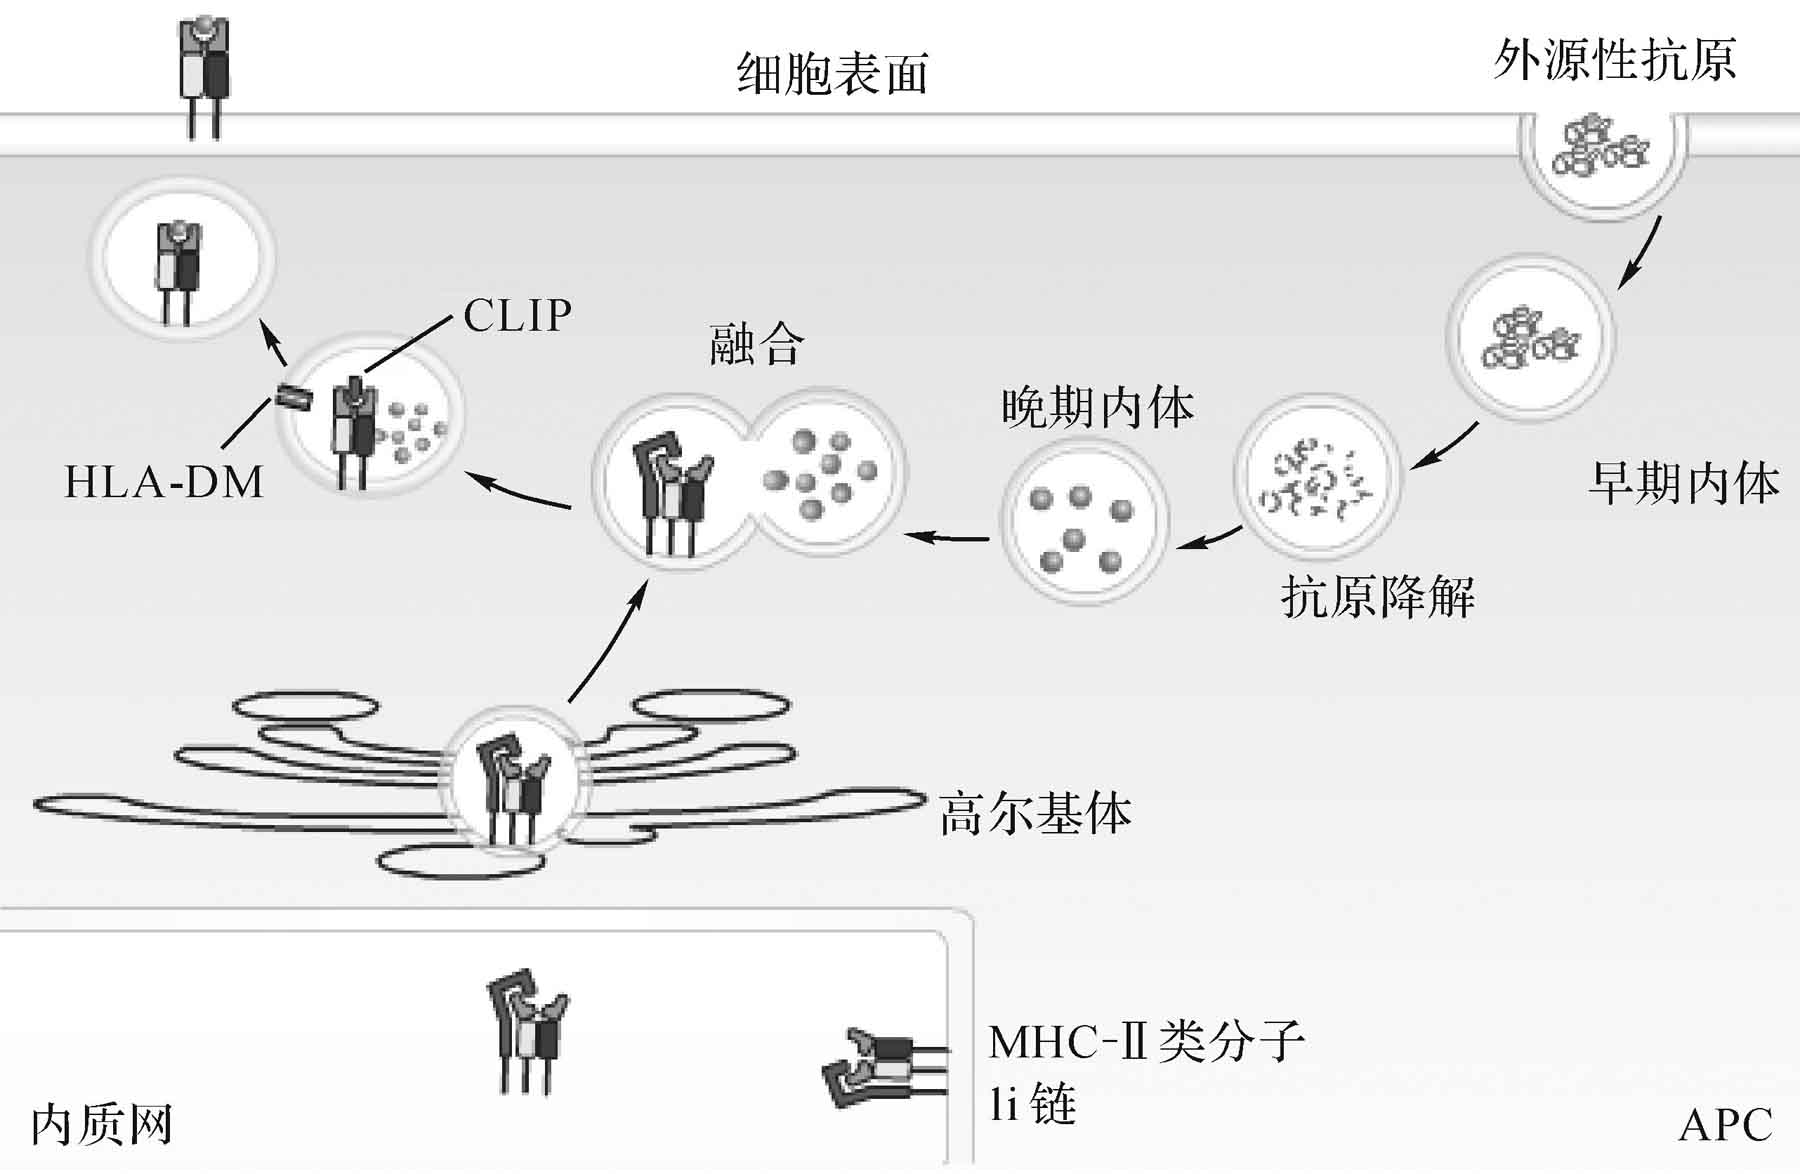
\includegraphics{./images/Image00133.jpg}
 \captionsetup{justification=centering}
 \caption{外源性抗原的加工、处理和递呈}
 \label{fig9-7}
  \end{figure} 

(二)MHC-Ⅱ类分子的生成和转运

MHC-Ⅱ类分子α链和β链在粗面ER中生成,并在钙联蛋白参与下折叠成异二聚体,插入粗面ER膜中。粗面ER膜上存在Ia相关的恒定链(Ia-associated
invariant
chain,Ii链),与MHC-Ⅱ类分子结合,形成九聚体(abIi)\textsubscript{3}
复合物。Ii链的作用是:①参与α链和β链折叠和组装,促进MHC-Ⅱ类分子二聚体形成;②阻止粗面ER中内源性肽与MHC-Ⅱ类分子结合;③促进MHC-Ⅱ类分子从ER移行,经高尔基体进入MIIC。

胞内合成的MHC-Ⅱ分子被高尔基体转运至一囊泡样腔室,后者称为MHC-Ⅱ类分子腔室(MHC
classIIcompartment,MIIC)。含外来抗原多肽的内体/溶酶体可与MIIC融合。随后,在酸性蛋白酶作用下,使与MHC-Ⅱ类分子结合的Ii链被部分降解,仅在MHC-Ⅱ类分子抗原肽结合槽中残留一小段,称为II类分子相关的恒定链多肽(classII-associated
invariant chainpeptide,CLIP)。

(三)MHC-Ⅱ类分子组装和递呈抗原肽

MHC-Ⅱ类分子的α\textsubscript{1} 和b\textsubscript{1}
功能区折叠为2个α螺旋和1个β片层,形成抗原肽结合沟槽,其两端为开放结构,使与之结合的多肽在N端及C端可适当延伸,最适的多肽长度在13~18个氨基酸之间。

存在于MIIC中的MHC-Ⅱ类分子,其抗原肽结合槽由CLIP占据,故不能与抗原肽结合。HLA-DM分子(属非经典MHC-Ⅱ类分子)可使CLIP与抗原肽结合沟槽离解,此时抗原肽才可与MHC-Ⅱ类分子结合为复合物。抗原肽-MHC-Ⅱ类分子复合物随MIIC向细胞表面移行,通过胞吐作用(exocytosis)而表达于细胞表面,供CD4\textsuperscript{+}
T细胞识别,完成外源性抗原肽递呈过程。


\subsection{内源性抗原的加工、处理和递呈}

(一)内源性抗原的加工处理和转运

胞内合成的内源性抗原在胞浆内被处理和转运。内源性抗原在多种酶和ATP的作用下与泛素结合,泛素化的内源性抗原被解除折叠,以线形进入蛋白酶体(proteosome)。蛋白酶体(20S)是存在于细胞内的一种大分子量蛋白质水解酶复合体,具有广泛的蛋白水解活性。蛋白酶体为中空(孔径约1~2nm)的圆柱体结构,内源性蛋白通过蛋白酶体的孔道,可被降解为含6~30个氨基酸的多肽片段。蛋白酶体由4个各含7个球形亚单位的圆环串接而成,其具有酶活性的组分主要是两种低分子量多肽(low
molecular weight
peptide,LMP),包括LMP2和LMP7(属于非经典MHC-Ⅱ类基因产物)(图\ref{fig9-8})。

\begin{figure}[!htbp]
 \centering
 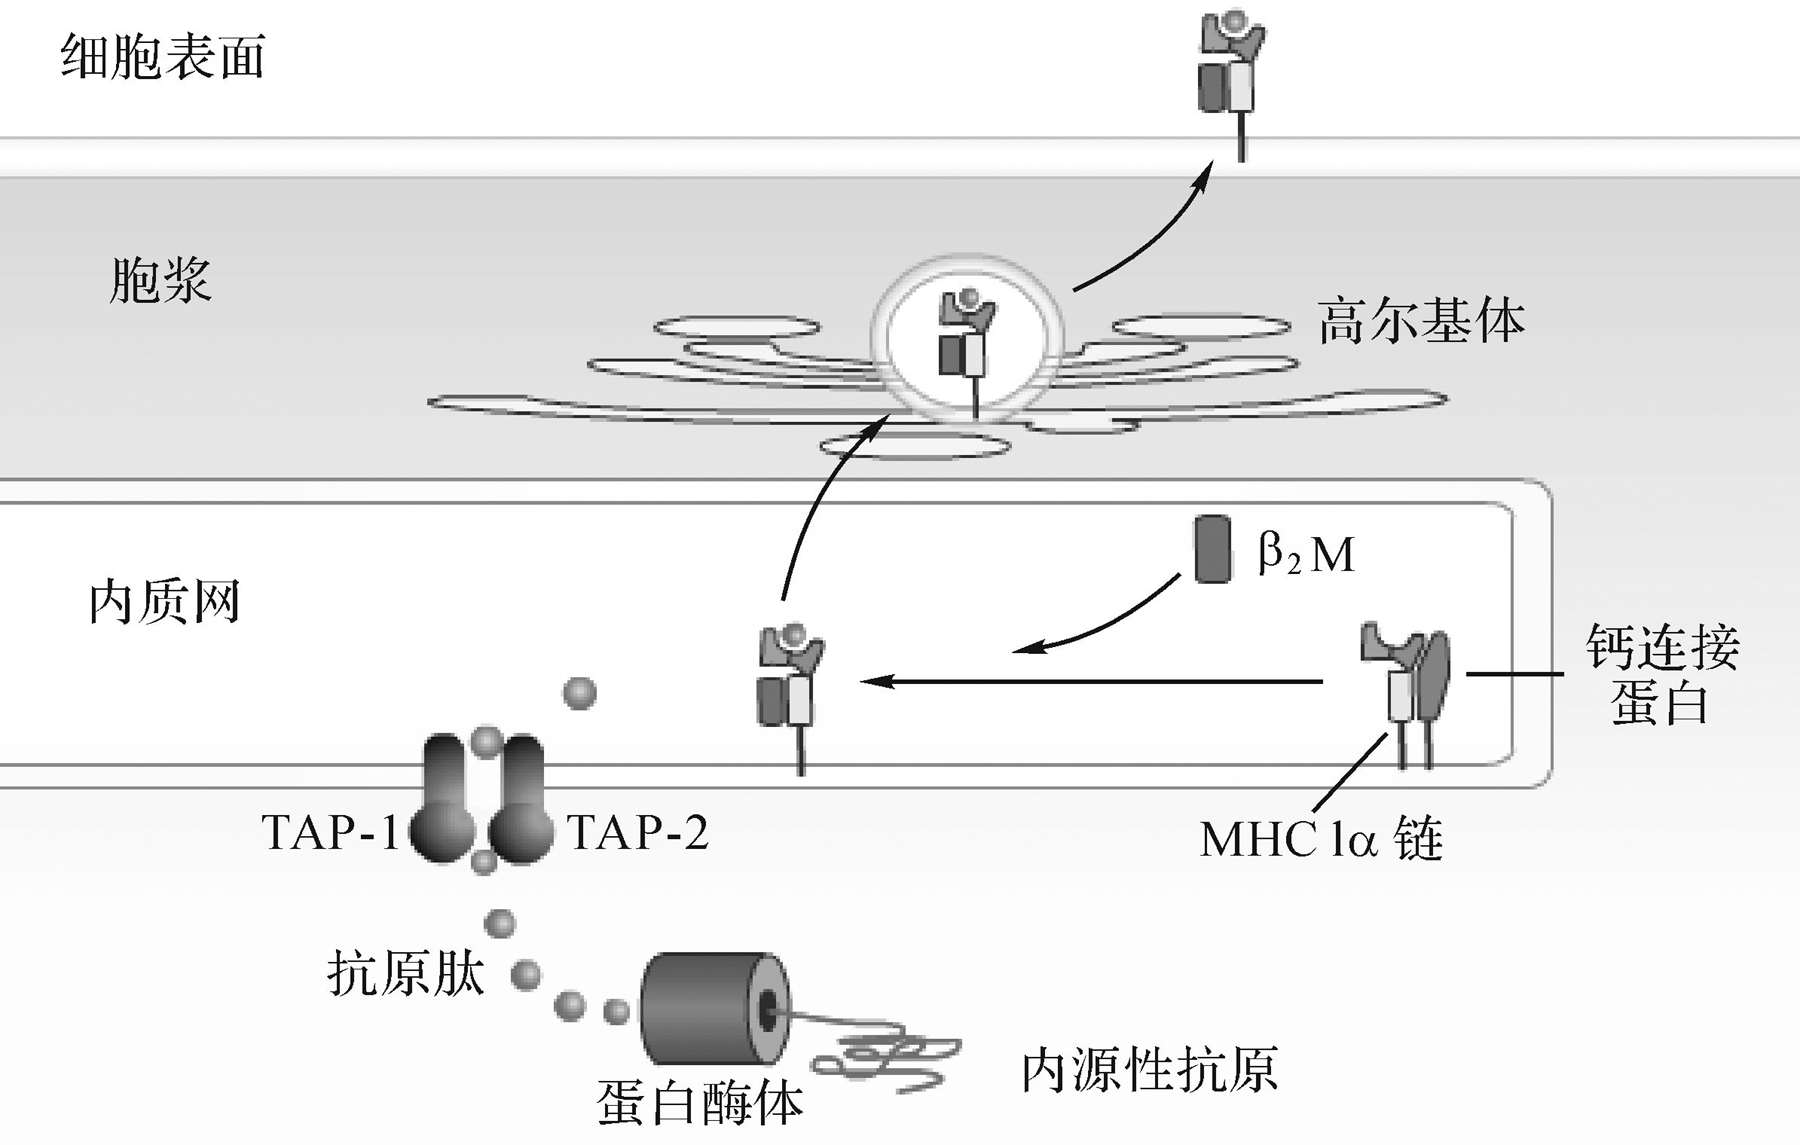
\includegraphics[width=.6\textwidth]{./images/Image00134.jpg}
 \captionsetup{justification=centering}
 \caption{内源性抗原的加工、处理和递呈}
 \label{fig9-8}
  \end{figure} 

经蛋白酶体降解的抗原肽片段须进入内质网(ER)才能与MHC-I类分子结合,该过程依赖于ER的抗原加工相关转运体(transporter
associated with antigen
processing,TAP)。TAP由TAP1和TAP2两个亚单位组成,是ER膜上的跨膜蛋白,各跨越ER膜6次,共同在ER膜上形成孔道。

胞浆中的抗原肽先与TAP的胞浆区结合,在TAP分子的ATP结合结构域作用下,使ATP降解,导致TAP异二聚体结构改变,孔道开放,抗原肽通过孔道进入ER腔。

TAP可选择性转运适合与MHC-I类分子结合的肽段,其机制为:①TAP能选择性转运含8~12个氨基酸、适合与MHC-I类分子结合的抗原肽;②TAP优先选择C端为碱性或疏水性残基的多肽片段,这些残基乃抗原肽与MHC-I类分子结合的锚着残基。

(二)MHC-I类分子的生成和组装

MHC-I类分子的重链(α链)和轻链(β2m)在粗面ER中合成后,被转运至光面ER。在ER中,MHC-I类分子须立即与某些伴随蛋白(chaperone)[如钙联蛋白(calnexin)、钙网蛋白(calreliculin)和tapasin]
结合。此类蛋白的作用是:参与α链的折叠及与β2m组装成完整的MHC-I类分子;保护α链不被降解;帮助MHC-I类分子与TAP结合。

(三)MHC-I类分子组装和递呈抗原肽

在伴随蛋白参与下,MHC-I类分子组装为二聚体,其 α链的α\textsubscript{1}
及α\textsubscript{2}
功能区构成抗原肽结合沟槽,沟槽的两个侧面为α螺旋,底面为β片层结构。MHC-I类分子沟槽纵向的两端是封闭的,能结合含8~12个氨基酸的多肽。

MHC-I类分子与ER上的TAP相连,再与经TAP转运的抗原肽结合,形成抗原肽-MHC-I类分子复合物,然后与TAP、伴随蛋白解离,移行至高尔基体,通过分泌囊泡再移行至细胞表面,递呈给CD8\textsuperscript{+}
T细胞。

\section{APC与T细胞的相互作用}

APC将抗原递呈给特异性T细胞,该过程涉及两种细胞表面多种分子间的相互作用,形成免疫突触(immune
synapse)。


\subsection{T细胞与APC的非特异性结合}

初始T细胞进入淋巴结皮质区深部,即与该处APC(成熟DC等)接触,T细胞表面的黏附分子(LFA-1、CD2、ICAM-3)与APC表面相应受体(ICAM-1或ICAM-2、LFA-3)短暂结合(图\ref{fig9-9})。这种非特异性、可逆性的结合,可为TCR提供机会,从APC表面大量抗原肽-MHC分子复合物中筛选特异性抗原肽。若未能遭遇特异性抗原,T细胞即与DC分离,离开淋巴结而进入血循环。

\begin{figure}[!htbp]
 \centering
 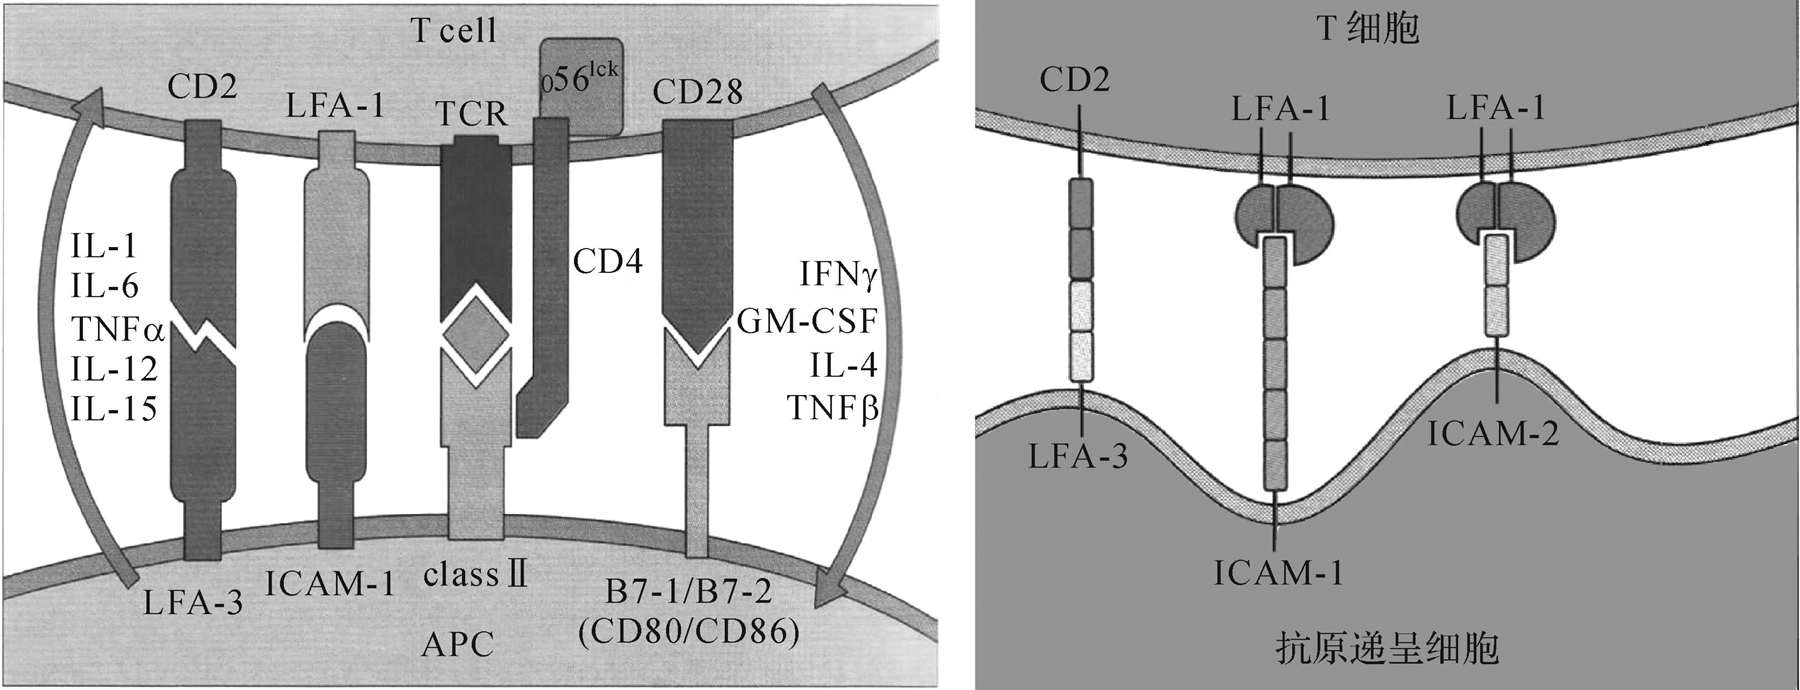
\includegraphics{./images/Image00135.jpg}
 \captionsetup{justification=centering}
 \caption{T细胞与APC的非特异性结合}
 \label{fig9-9}
  \end{figure} 


\subsection{T细胞与APC的特异性结合}

上述APC与T细胞短暂结合过程中,若TCR遭遇特异性抗原肽,则T细胞与APC发生特异性结合,并由CD3分子向胞内传递特异性识别信号,导致LFA-1变构并增强其与ICAM的亲和力,从而稳定并延长APC与T细胞间的接触(可持续数天),以有效诱导抗原特异性T细胞激活和增殖。增殖的子代细胞仍与APC黏附,直至分化为效应细胞。

此外,在T细胞与APC的特异性结合中,T细胞表面CD4与CD8分子是TCR识别抗原的共受体(co-receptor)。CD4和CD8可分别与APC(或靶细胞)表面MHC-Ⅱ和MHC-Ⅰ类分子结合,从而增强TCR与特异性抗原肽-MHC分子复合物结合的亲和力,使T细胞对抗原应答的敏感性增强(约100倍)(图\ref{fig9-10})。

\begin{figure}[!htbp]
 \centering
 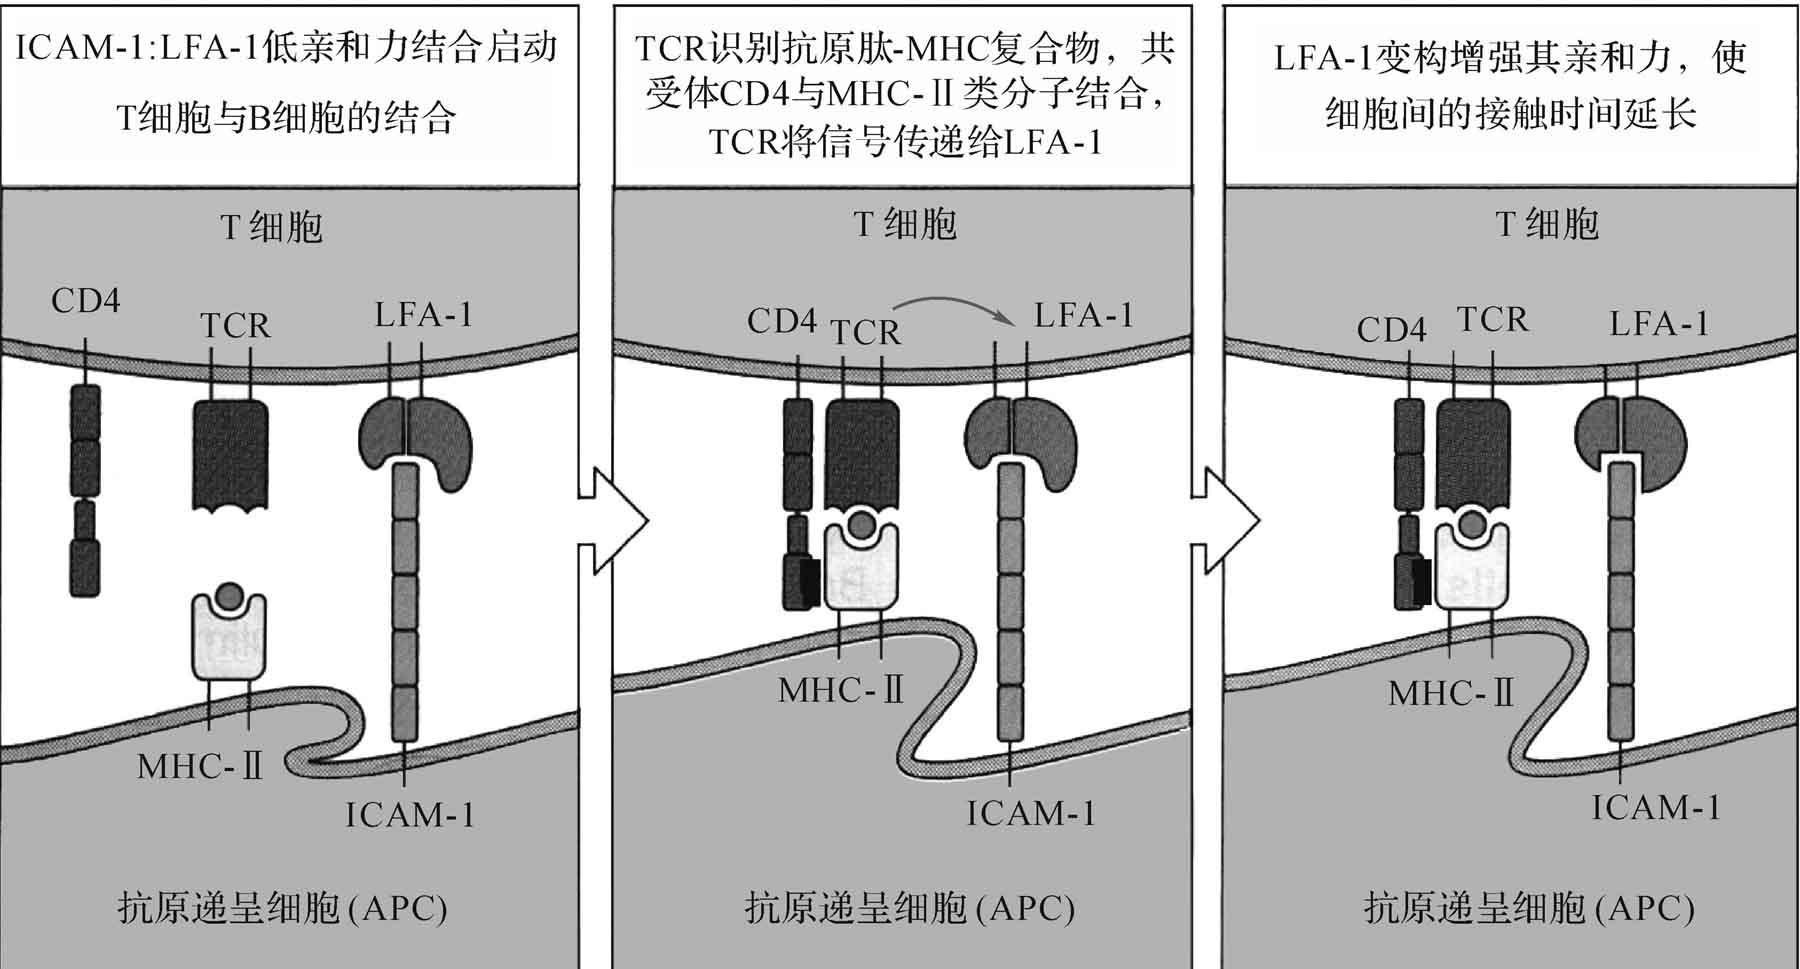
\includegraphics{./images/Image00136.jpg}
 \captionsetup{justification=centering}
 \caption{TCR与APC的特异性稳定结合}
 \label{fig9-10}
  \end{figure} 


\subsection{T细胞和APC表面共刺激分子的结合}

APC和T细胞表面均表达多种参与两类细胞相互作用的黏附分子对,又称共刺激分子(co-stimulatory
molecule),它们的结合有助于维持、加强APC与T细胞的直接接触,并为T细胞激活提供共刺激信号(co-stimulatory
signal)。


\subsection{T细胞活化、增殖和分化}

通常情况下,体内表达某一特异性TCR的T细胞克隆仅占总T细胞库的1/10\textsuperscript{5}
~1/10\textsuperscript{4}
。数量极少的特异性T细胞仅在被抗原激活后,通过克隆扩增而产生大量效应细胞,才能有效发挥作用。

(一)T细胞活化

接受抗原刺激后,T细胞的完全活化有赖于双信号和细胞因子的作用(图\ref{fig9-11})。

\begin{figure}[!htbp]
 \centering
 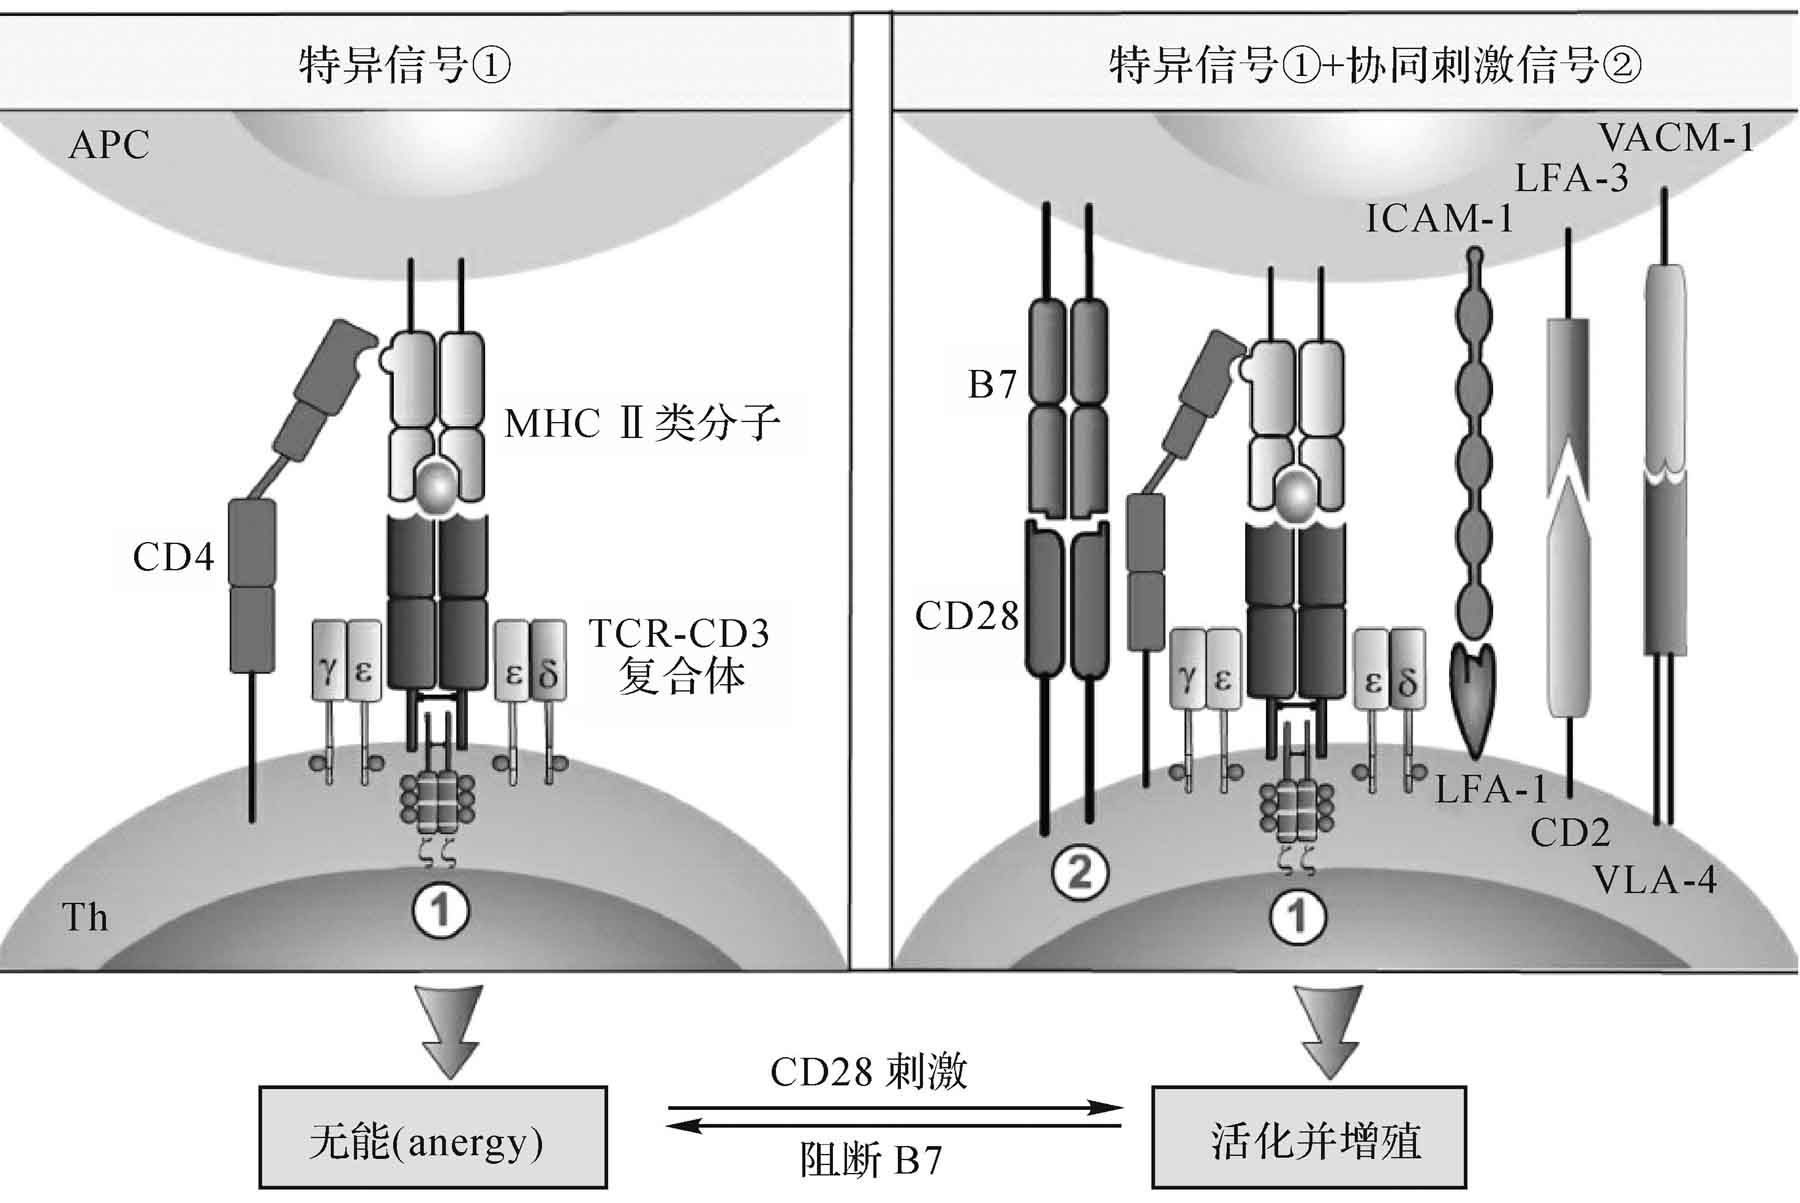
\includegraphics{./images/Image00137.jpg}
 \captionsetup{justification=centering}
 \caption{T细胞活化相关信号分子}
 \label{fig9-11}
  \end{figure} 

1.T细胞活化的第一信号

APC将抗原肽-MHC分子复合物递呈给T细胞,TCR特异性识别结合于MHC分子凹槽中的抗原肽,引起TCR交联并启动抗原识别信号(即第一信号),导致CD3和共受体(CD4或CD8)分子的胞浆段尾部相聚,激活与胞浆段尾部相连的酪氨酸激酶,促使含酪氨酸的蛋白磷酸化,启动激酶活化的级联反应,最终通过激活转录因子而导致细胞因子及其受体等的基因转录和产物合成。

2.T细胞激活的第二信号

仅有TCR来源的抗原识别信号尚不足以有效激活T细胞。APC和T细胞表面多种黏附分子对(如B7/CD28、LFA-1/ICAM-1或ICAM-2、CD2/LFA-3等)结合,可向T细胞提供第二激活信号(即共刺激信号),从而使T细胞完全活化。

CD28/B7是重要的共刺激分子,其主要作用是促进IL-2合成。在缺乏共刺激信号的情况下,IL-2合成受阻,则抗原刺激非但不能激活特异性T细胞,反而导致T细胞失能(anergy)。激活的专职APC高表达共刺激分子,而正常组织及静止的APC则不表达或仅低表达共刺激分子。缺乏共刺激信号使自身反应性T细胞处于无能状态,从而有利于维持自身耐受。

此外,CTLA4与CD28具有高度同源性,该分子与B7的亲和力比CD28高约20倍。CD28/B7参与T细胞的激活,但在T细胞激活至峰值后CTLA4表达则增加,后者与B7结合可启动抑制性信号,从而有效制约特异性T细胞克隆过度增殖(图\ref{fig9-12})。

\begin{figure}[!htbp]
 \centering
 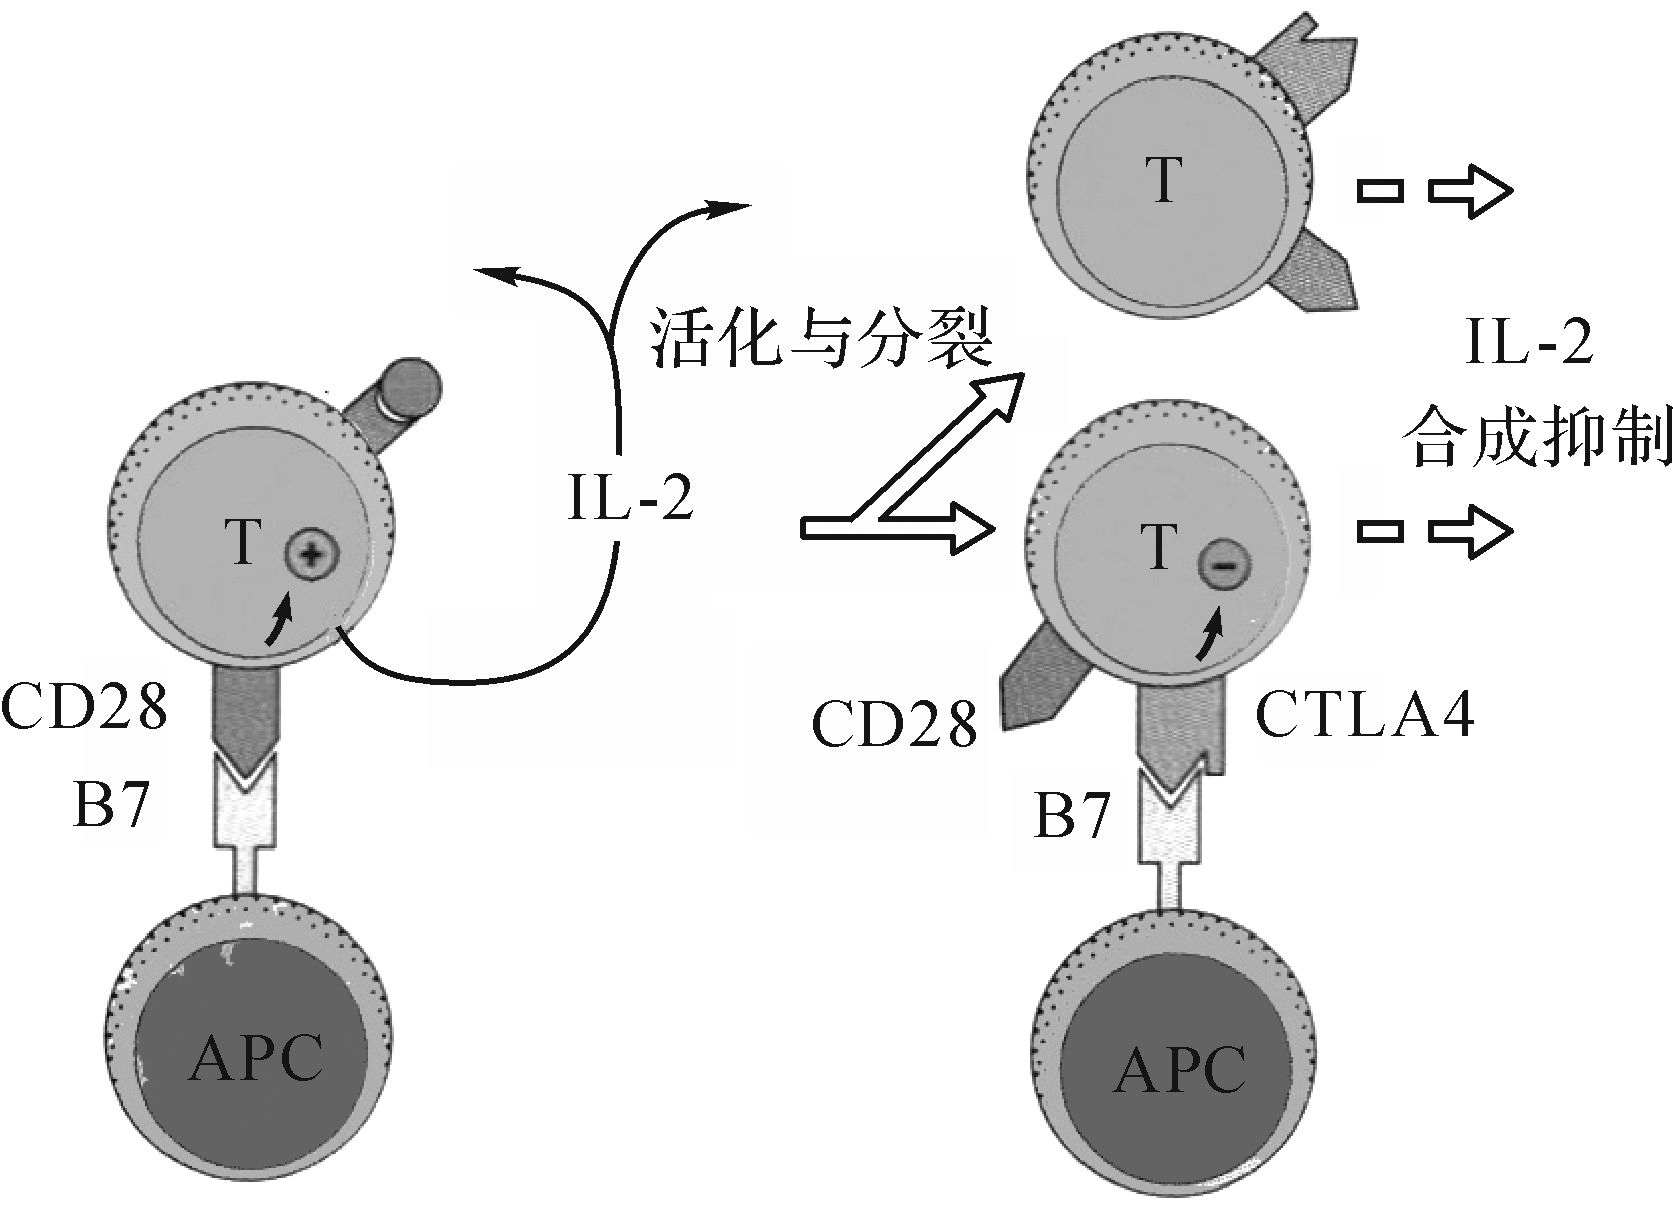
\includegraphics[width=.5\textwidth]{./images/Image00138.jpg}
 \captionsetup{justification=centering}
 \caption{CD28/B7和CTLA4/B7介导的不同效应}
 \label{fig9-12}
  \end{figure} 

3.细胞因子促进T细胞充分活化

除上述双信号外,T细胞的充分活化还有赖于细胞因子参与。活化的APC和T细胞可分泌IL-1、IL-2、IL-6,IL-12等多种细胞因子,它们在T细胞激活中发挥重要作用。

(二)T细胞增殖和分化

1.T细胞增殖、分化及其机制

激活的T细胞迅速进入细胞周期,通过有丝分裂而大量增殖,并分化为效应T细胞,然后离开淋巴器官随血循环到达感染部位。多种细胞因子参与T细胞增殖和分化过程,其中最重要者为IL-2。IL-2受体由α、β、γ链组成,静止T细胞仅表达低亲和力IL-2R(β.γ);激活的T细胞可表达高亲和力IL-2R(α.β.γ)并分泌IL-2。通过自分泌及旁分泌作用,IL-2与T细胞表面IL-2R结合,介导T细胞增殖和分化。此外,IL-4、IL-12、IL-15等细胞因子也在T细胞增殖和分化中(尤其Th1与Th2细胞的分化调控中)发挥重要作用。T细胞的增殖、分化如图\ref{fig9-13}所示。

\begin{figure}[!htbp]
 \centering
 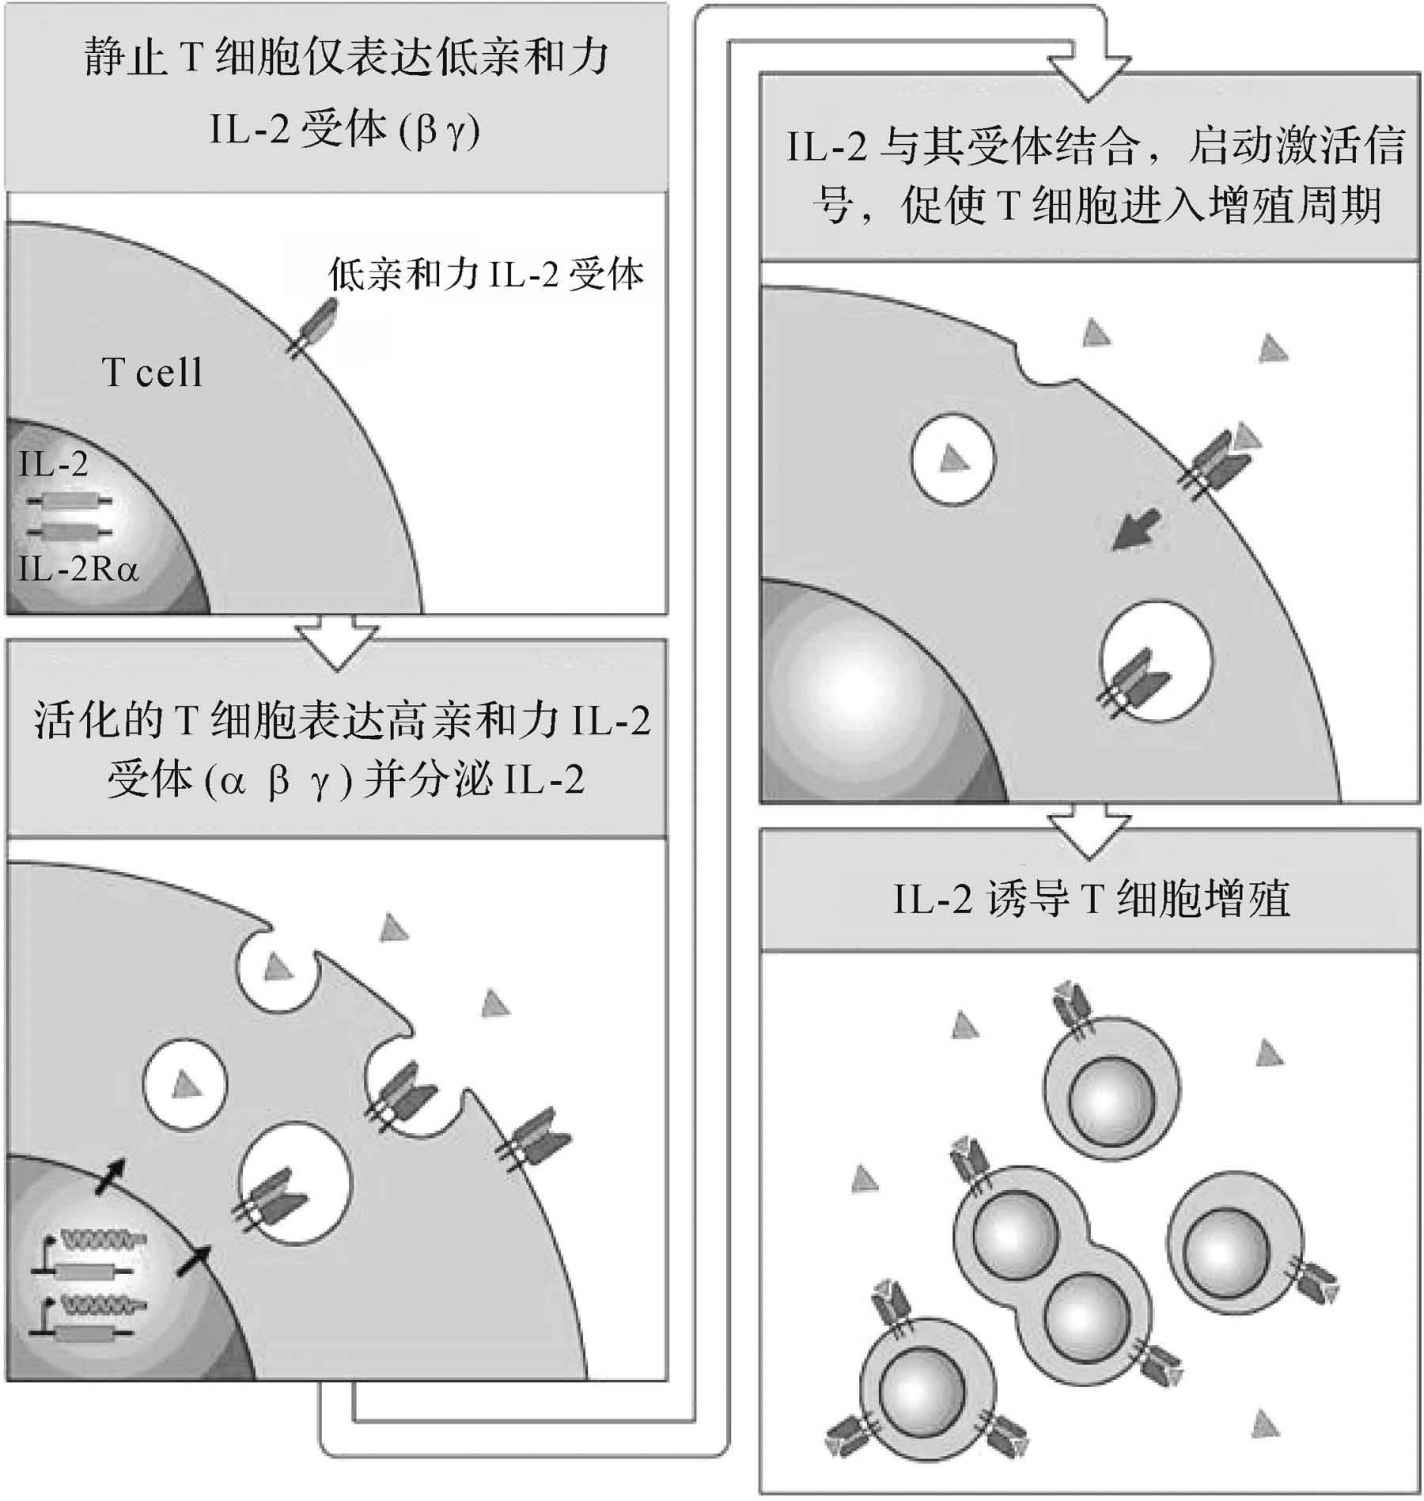
\includegraphics{./images/Image00139.jpg}
 \captionsetup{justification=centering}
 \caption{T细胞的增殖、分化}
 \label{fig9-13}
  \end{figure} 

T细胞经迅速增殖4-5天后,分化为可高表达效应分子(包括膜分子和分泌型细胞因子等)的效应T细胞(Th细胞或CTL)。同时,部分活化的T细胞可分化为长寿命记忆性T细胞,在再次免疫应答中起重要作用。

2.CD4\textsuperscript{+} T细胞的增殖分化

初始CD4\textsuperscript{+}
T被激活、增殖和分化为Th0细胞。局部微环境中存在的细胞因子种类是调控Th0细胞分化的关键因素,例如:IL-12可促进Th0细胞定向分化为Th1细胞;IL-4可促进Th0细胞分化为Th2细胞。Th0细胞的分化方向是决定机体免疫应答类型的重要因素:Th1细胞主要介导细胞免疫应答;Th2细胞主要介导体液免疫应答。

3.CD8\textsuperscript{+} T细胞的增殖和分化

初始CD8\textsuperscript{+} T细胞的激活主要有两种方式:

(1)Th细胞非依赖性:如病毒感染的DC,由于其高表达共刺激分子,可直接刺激CD8\textsuperscript{+}
T细胞合成IL-2,促使CD8\textsuperscript{+}
T细胞自身增殖并分化为细胞毒T细胞,而无需Th细胞辅助。

(2)Th细胞依赖性:CD8\textsuperscript{+}
T细胞作用的靶细胞一般仅低表达或不表达共刺激分子,不能激活初始CD8\textsuperscript{+}
T细胞,而需要APC及CD4\textsuperscript{+} T细胞的辅助。

(三)活化T细胞的转归

1.活化T细胞转变为记忆T细胞,参与再次免疫应答

机体对特定抗原产生初次免疫应答后,部分活化的T细胞可转变为记忆T细胞(Tm)。当抗原再次进入机体,仅需少量抗原即可激活Tm,迅速产生强烈、持久的应答。

2.活化T细胞发生凋亡,以及时终止免疫应答

活化的淋巴细胞发生凋亡有助于控制免疫应答强度,以适时终止免疫应答和维持自身免疫耐受。活化淋巴细胞凋亡涉及两条途径(图\ref{fig9-14})。

\begin{figure}[!htbp]
 \centering
 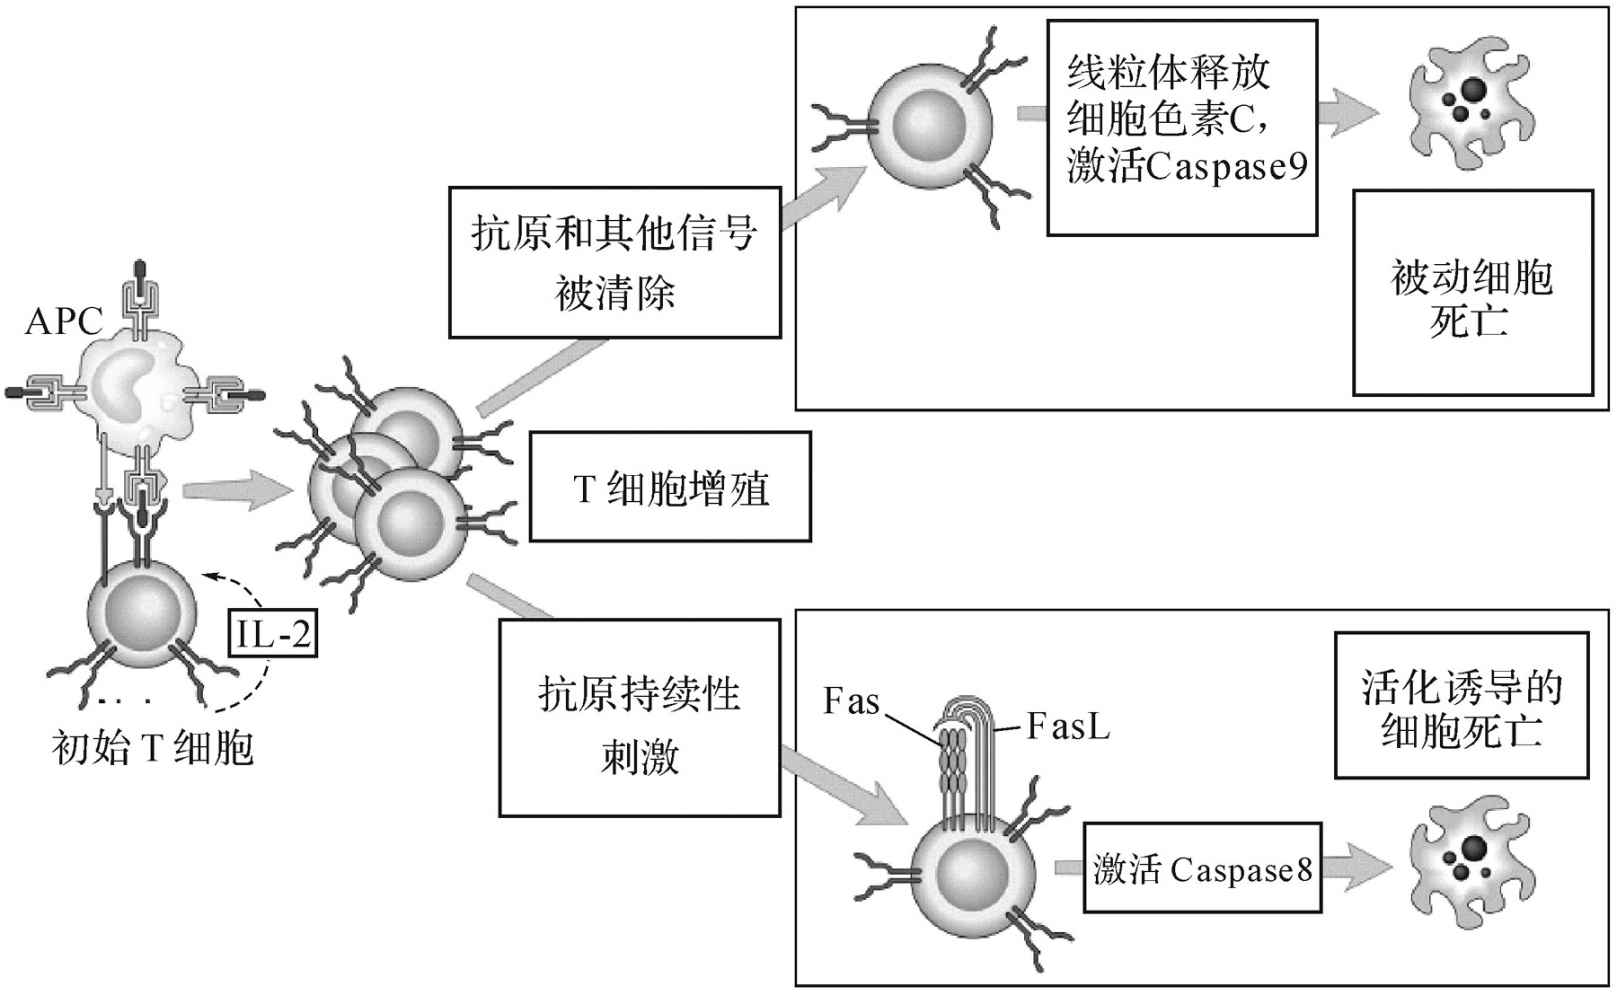
\includegraphics[width=.6\textwidth]{./images/Image00140.jpg}
 \captionsetup{justification=centering}
 \caption{活化T细胞的凋亡}
 \label{fig9-14}
  \end{figure} 

(1)活化诱导的细胞死亡(activation induced cell
death,AICD):激活的T细胞可高表达死亡受体Fas及Fas配体(Fas
ligand,FasL),二者结合后可启动Caspase酶联反应而导致细胞凋亡。AICD有助于控制特异性T细胞克隆的扩增水平,从而发挥重要的负向免疫调节作用。

(2)被动细胞死亡(passive cell
death,PCD):在免疫应答晚期,由于大量抗原被清除,淋巴细胞所接受的抗原刺激和生存信号及所产生的生长因子均减少,导致胞内线粒体释放细胞色素C,通过Caspase酶联反应而致细胞凋亡。

\section{B细胞介导的体液免疫应答}

许多引起感染性疾病的细菌存在于细胞外,同时多数胞内寄生病原体的传播是通过细胞外间隙从一个细胞转移至另一细胞。这些存在于细胞外的病原体主要由B细胞介导的体液免疫应答进行清除。

成熟的初始B细胞离开骨髓进入外周循环,这些细胞若未遭遇相应抗原,即在数周内死亡;若遭遇特异性抗原,则发生活化、增殖,并分化成浆细胞,通过产生和分泌抗体而发挥清除病原体的作用。在B细胞应答中,由浆细胞所产生的抗体(存在于体液中)是主要的效应分子,故将此类应答称为体液免疫应答(humoral
immunity)。

B细胞应答的过程随刺激机体的抗原种类不同而各异。在TD抗原刺激下,B细胞应答依赖Th细胞辅助(通常为Th2细胞);在TI抗原刺激下,B细胞可直接产生应答。


\subsection{B细胞对抗原的识别}

(一)B细胞对TI抗原的识别

细菌多糖、多聚鞭毛蛋白、脂多糖等属胸腺非依赖性抗原(TI抗原),其主要特征是不易降解,能激活初始B细胞而无需Th细胞辅助。TI抗原主要激活CD5\textsuperscript{+}
B1细胞,所产生的抗体主要为IgM。此类B细胞应答不受MHC限制,亦无需APC和Th细胞辅助。一般而言,由于无特异性T细胞辅助,TI抗原不能诱导抗体类型转换、抗体亲和力成熟和记忆性B细胞形成(即无免疫记忆)。

高剂量TI抗原(如LPS)可非特异性激活多克隆B细胞,故将其称为B细胞丝裂原。但是,低剂量TI-1抗原(为多克隆激活剂量的10\textsuperscript{-3}
-10\textsuperscript{-5}
)仅激活表达特异性BCR的B细胞,因为此类B细胞的BCR可从低浓度抗原中竞争性结合到足以激活自身的抗原量(图\ref{fig9-15})。

\begin{figure}[!htbp]
 \centering
 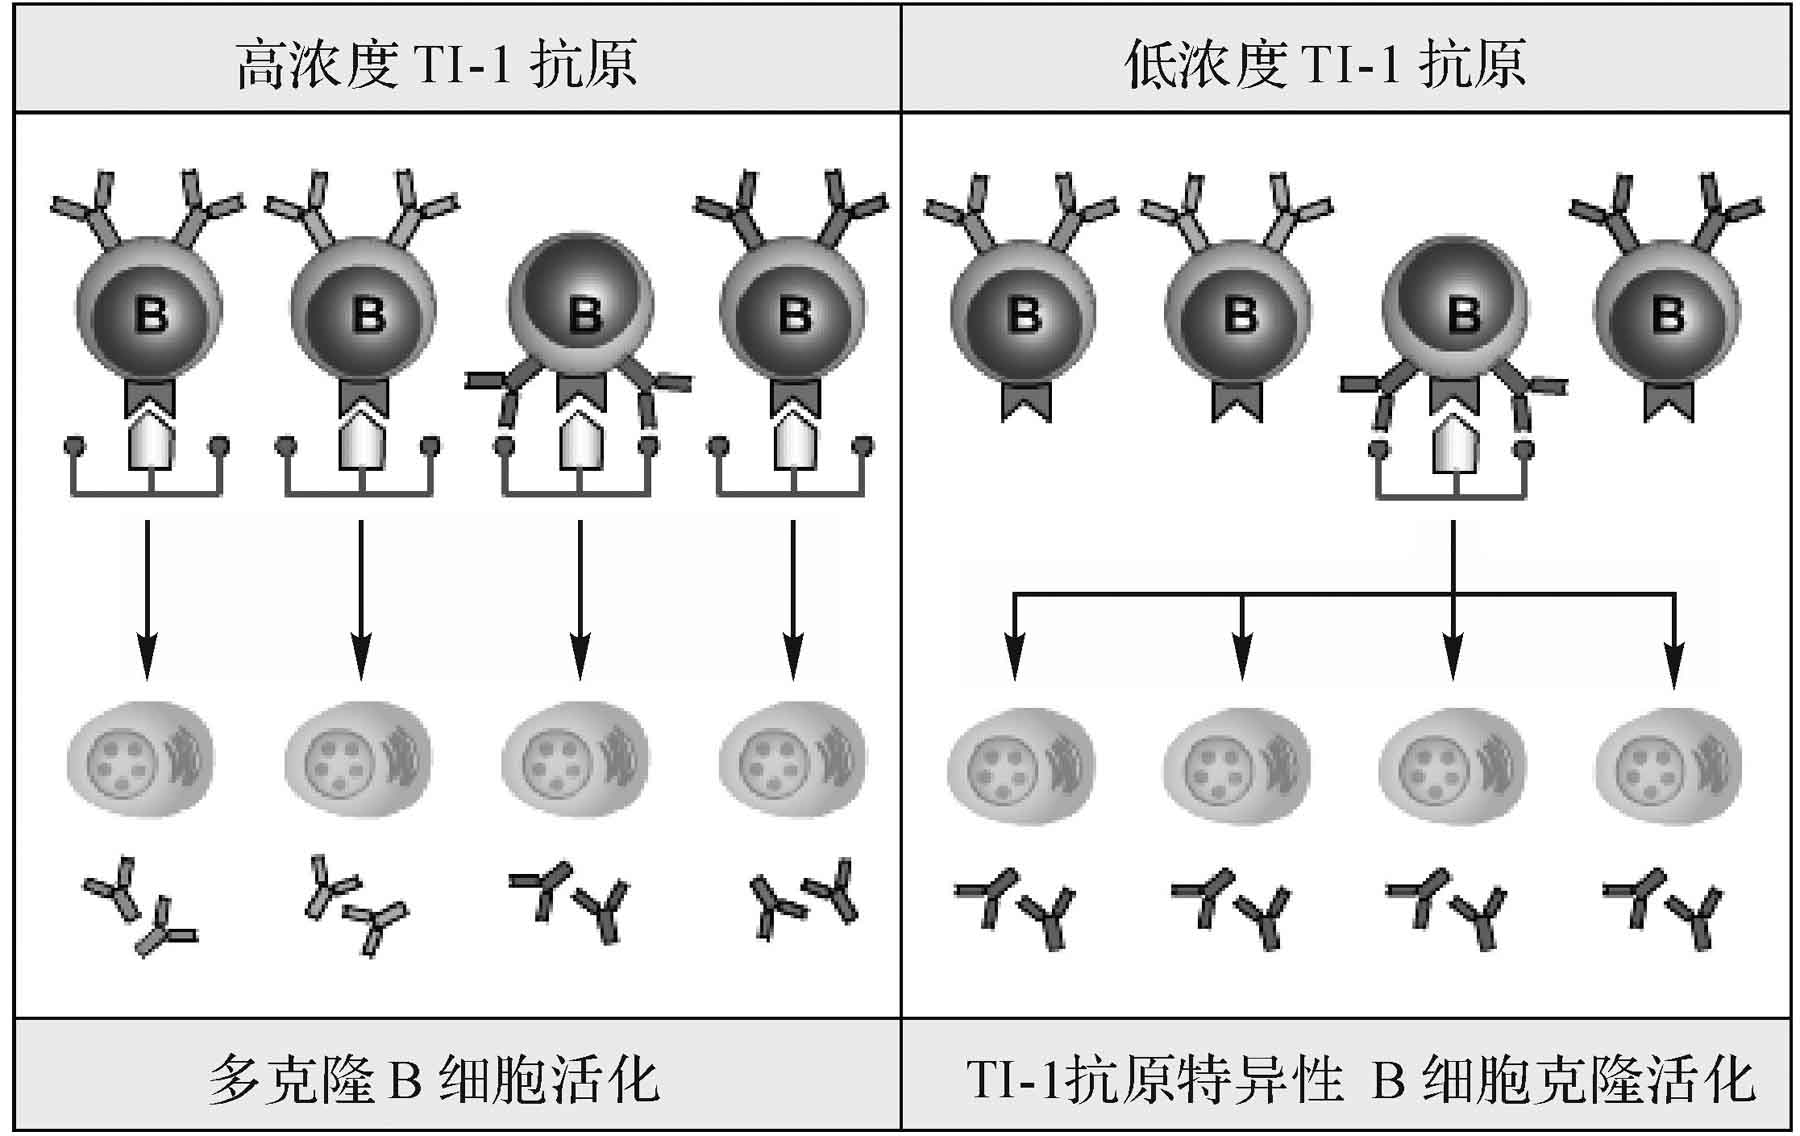
\includegraphics{./images/Image00141.jpg}
 \captionsetup{justification=centering}
 \caption{TI抗原诱导B细胞的激活}
 \label{fig9-15}
  \end{figure} 

(二)B细胞对TD抗原的识别

B细胞针对TD抗原的应答需抗原特异性T细胞辅助(图\ref{fig9-16})。与TCR不同,BCR分子可变区能直接识别天然抗原决定基,而无需APC对抗原的处理和递呈。必须指出的是,虽然抗原特异性B细胞与Th细胞所识别的表位不同,但二者须识别同一抗原分子的不同表位,才能相互作用。

\begin{figure}[!htbp]
 \centering
 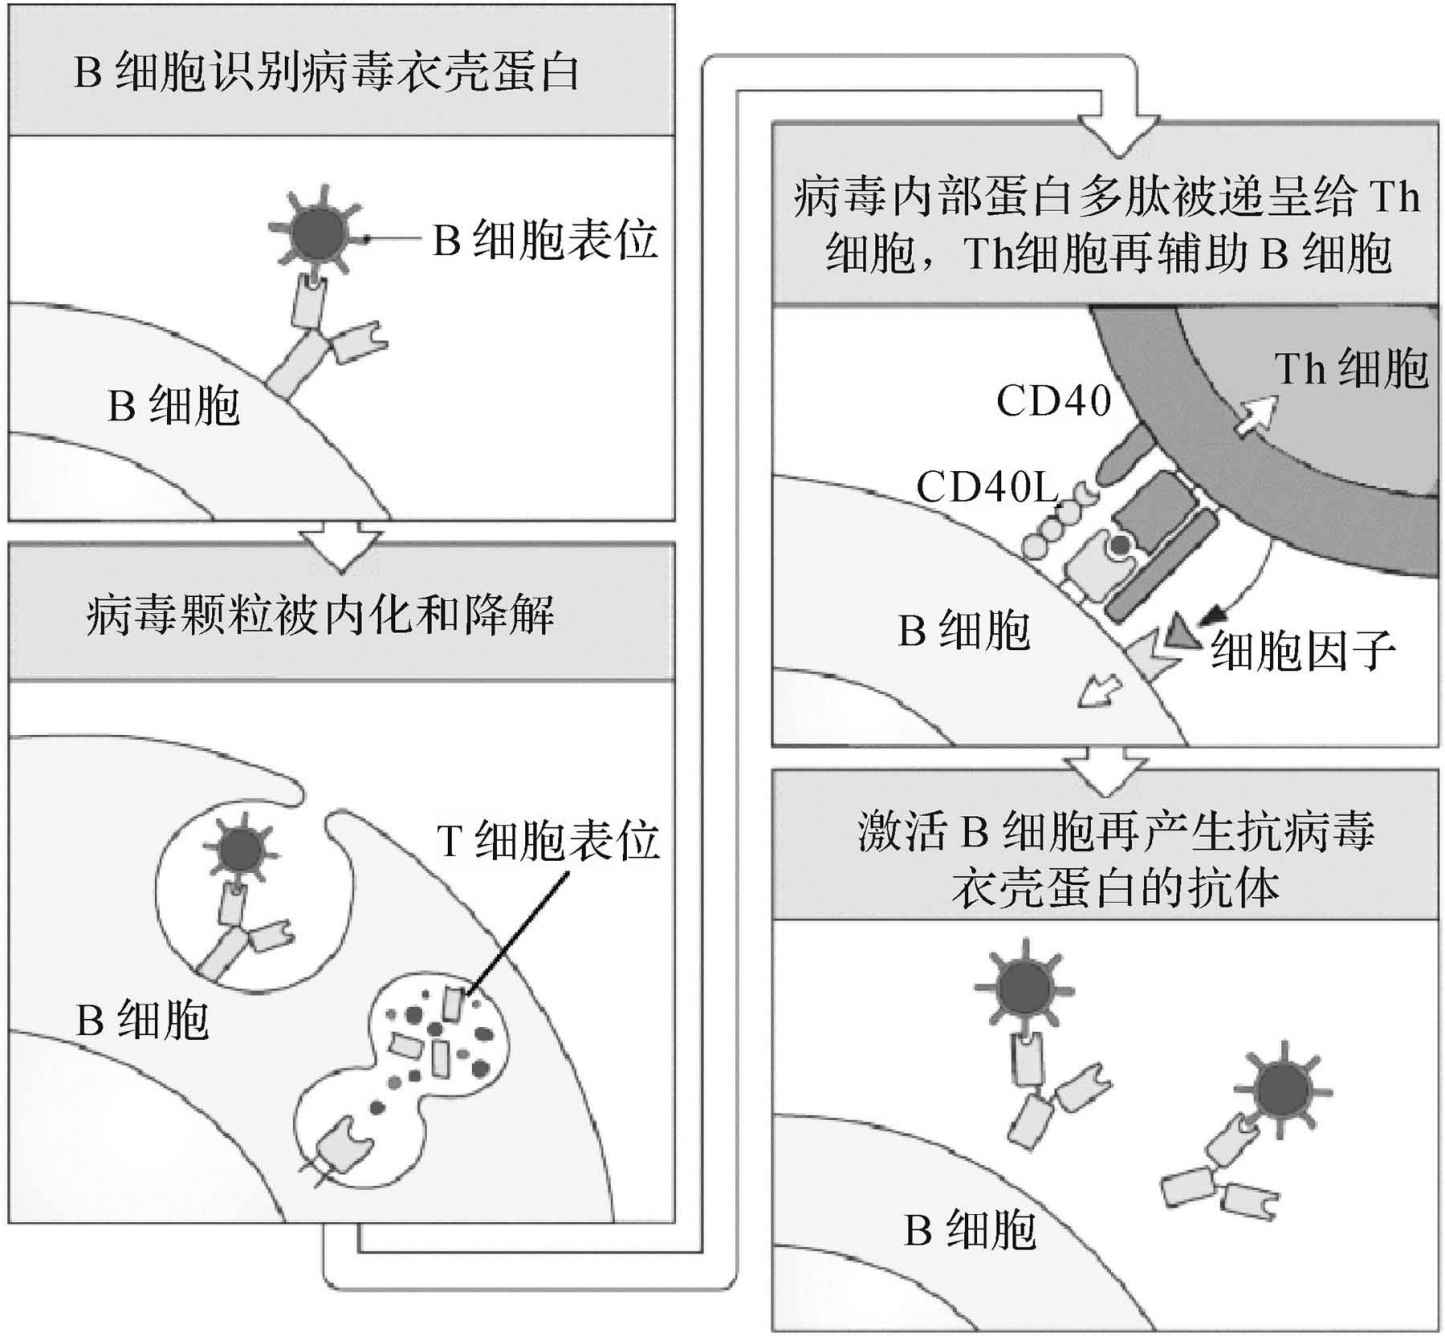
\includegraphics{./images/Image00142.jpg}
 \captionsetup{justification=centering}
 \caption{B细胞对TD抗原的识别}
 \label{fig9-16}
  \end{figure} 

BCR识别抗原对B细胞激活有两个作用:①BCR特异性结合抗原,向B细胞内传递抗原刺激信号;②BCR特异性结合抗原,通过内化作用将其摄入胞内,并将抗原降解为肽段,形成抗原肽-MHC-Ⅱ类分子复合物,供抗原特异性Th细胞识别。


\subsection{B细胞活化、增殖和分化}

(一)B细胞活化

与T细胞相似,B细胞活化也需要双信号和细胞因子参与。

1.B细胞激活的特异性抗原识别信号(第一信号)

BCR与特异性抗原表位结合,启动第一信号,并由Igα/Igβ将信号传入B细胞内。B细胞表面的BCR共受体复合物(CD21-CD19-CD81)在B细胞活化中发挥如下重要作用:①可使B细胞对抗原刺激的敏感性明显增强;②对结合有补体片段的免疫复合物或抗原,BCR可特异性识别其中的抗原组分,而BCR共受体
的CD21可与补体片段(如C3d)结合,通过受体/共受体交联,使CD19胞内段相连的酪氨酸激酶和Igα/Igβ;相关的酪氨酸激酶发生磷酸化,通过一系列级联反应,促进相关基因表达,使B细胞激活和增殖(图\ref{fig9-17})。

\begin{figure}[!htbp]
 \centering
 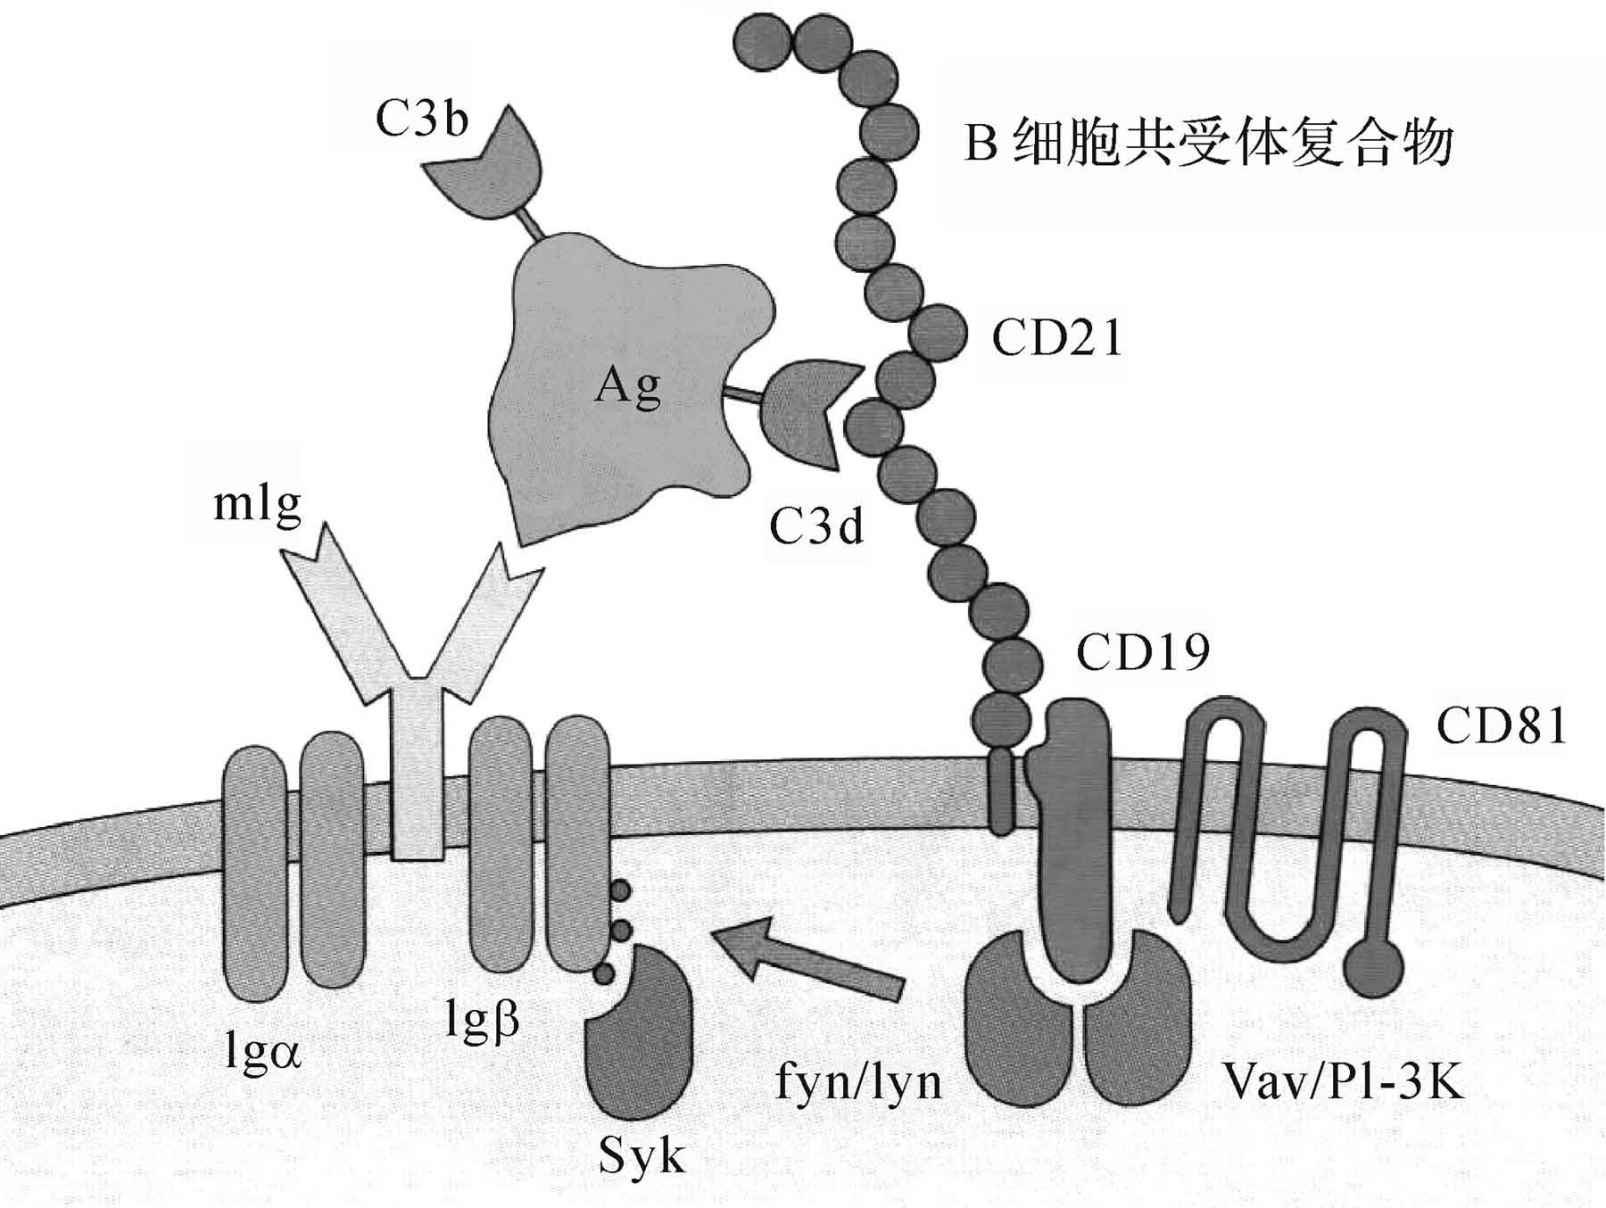
\includegraphics{./images/Image00143.jpg}
 \captionsetup{justification=centering}
 \caption{B细胞激活的第一信号}
 \label{fig9-17}
  \end{figure} 

2.B细胞激活的共刺激信号(第二信号)

B细胞激活有赖于T细胞辅助,通过B细胞与Th细胞间复杂的相互作用,B细胞获得其活化所必需的共刺激信号。

(1)初始Th细胞激活:初始Th细胞特异性识别APC(主要是DC)所递呈的抗原肽-MHC-Ⅱ类分子复合物而被激活,在外周淋巴组织(如淋巴结等)的T细胞区增殖,并分化为效应Th细胞。

(2)Th细胞与特异性B细胞的结合:循环中的B细胞进入外周淋巴组织后,多数未受抗原刺激的B细胞迅速穿越T细胞区进入B细胞区(初级淋巴滤泡)。已被抗原刺激的特异性B细胞,与相应的抗原特异性Th细胞相遇,被阻留在T细胞区,并发生复杂的相互作用:①Th细胞的TCR特异性识别并结合B细胞表面抗原肽-MHC-Ⅱ类分子复合物,由此,T细胞和B细胞识别同一抗原的不同表位;②效应Th细胞与B细胞表面的多种黏附分子对(如LFA3/CD2、ICAM-1或-3/LFA1、MHC-Ⅱ类分子/CD4等)相互作用,使T细胞与B细胞的特异性结合更为牢固。

(3)特异性B细胞活化:效应Th细胞识别B细胞递呈的特异性抗原,诱导性表达多种膜分子,其中最重要者为CD40L。Th细胞表面CD40L可与B细胞表面CD40结合,是向B细胞提供共刺激信号的最重要分子对,其主要效应为:促进B细胞进入增殖周期;上调B细胞表达B7分子,以增强B细胞对Th细胞的激活作用;促进生发中心发育及抗体类别转换。

3.细胞因子的作用

巨噬细胞分泌的IL-1和Th2细胞分泌的IL-4等细胞因子也参与B细胞活化,诱导B细胞依次表达IL-2R及其他细胞因子受体,与Th细胞分泌的相应细胞因子发生反应。细胞因子的参与是B细胞充分活化和增殖的必要条件。细胞因子在B细胞活化中的作用如图\ref{fig9-18}所示。

\begin{figure}[!htbp]
 \centering
 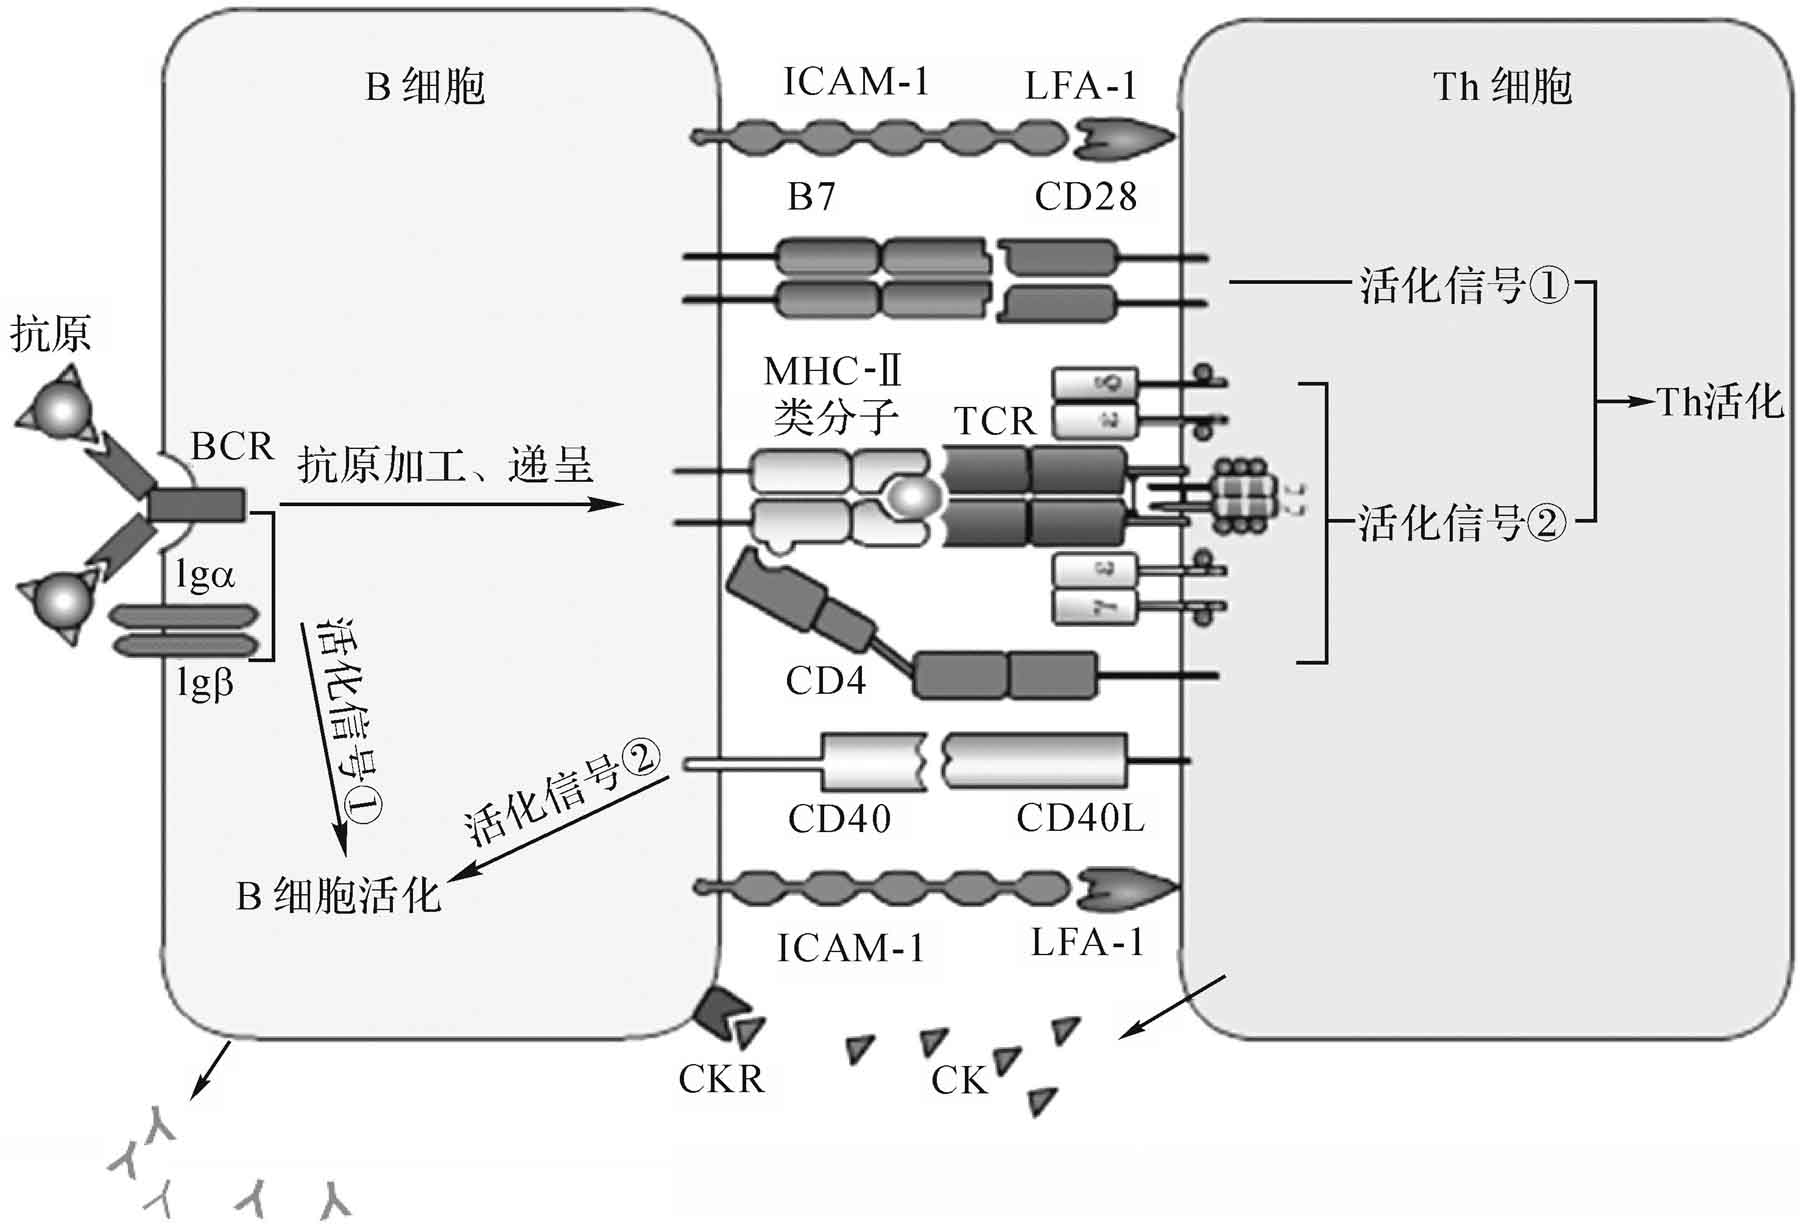
\includegraphics{./images/Image00144.jpg}
 \captionsetup{justification=centering}
 \caption{细胞因子在B细胞活化中的作用}
 \label{fig9-18}
  \end{figure} 

(二)B细胞的增殖、分化

活化的B细胞表面表达多种细胞因子受体,可响应Th细胞所分泌细胞因子的作用。其中,IL-2、IL-4和IL-5可促进B细胞增殖;IL-5、IL-6等可促进B细胞分化为能产生抗体的浆细胞(plasma
cell,PC),一部分B细胞分化转化为记忆性B细胞(memory B
cell)。记忆性B细胞为长寿命、低增殖细胞,其表达膜Ig,但不能大量产生抗体,一旦再次遭遇同一特异性抗原,即迅速活化、增殖、分化,产生大量高亲和力特异性抗体(图\ref{fig9-19})。

\begin{figure}[!htbp]
 \centering
 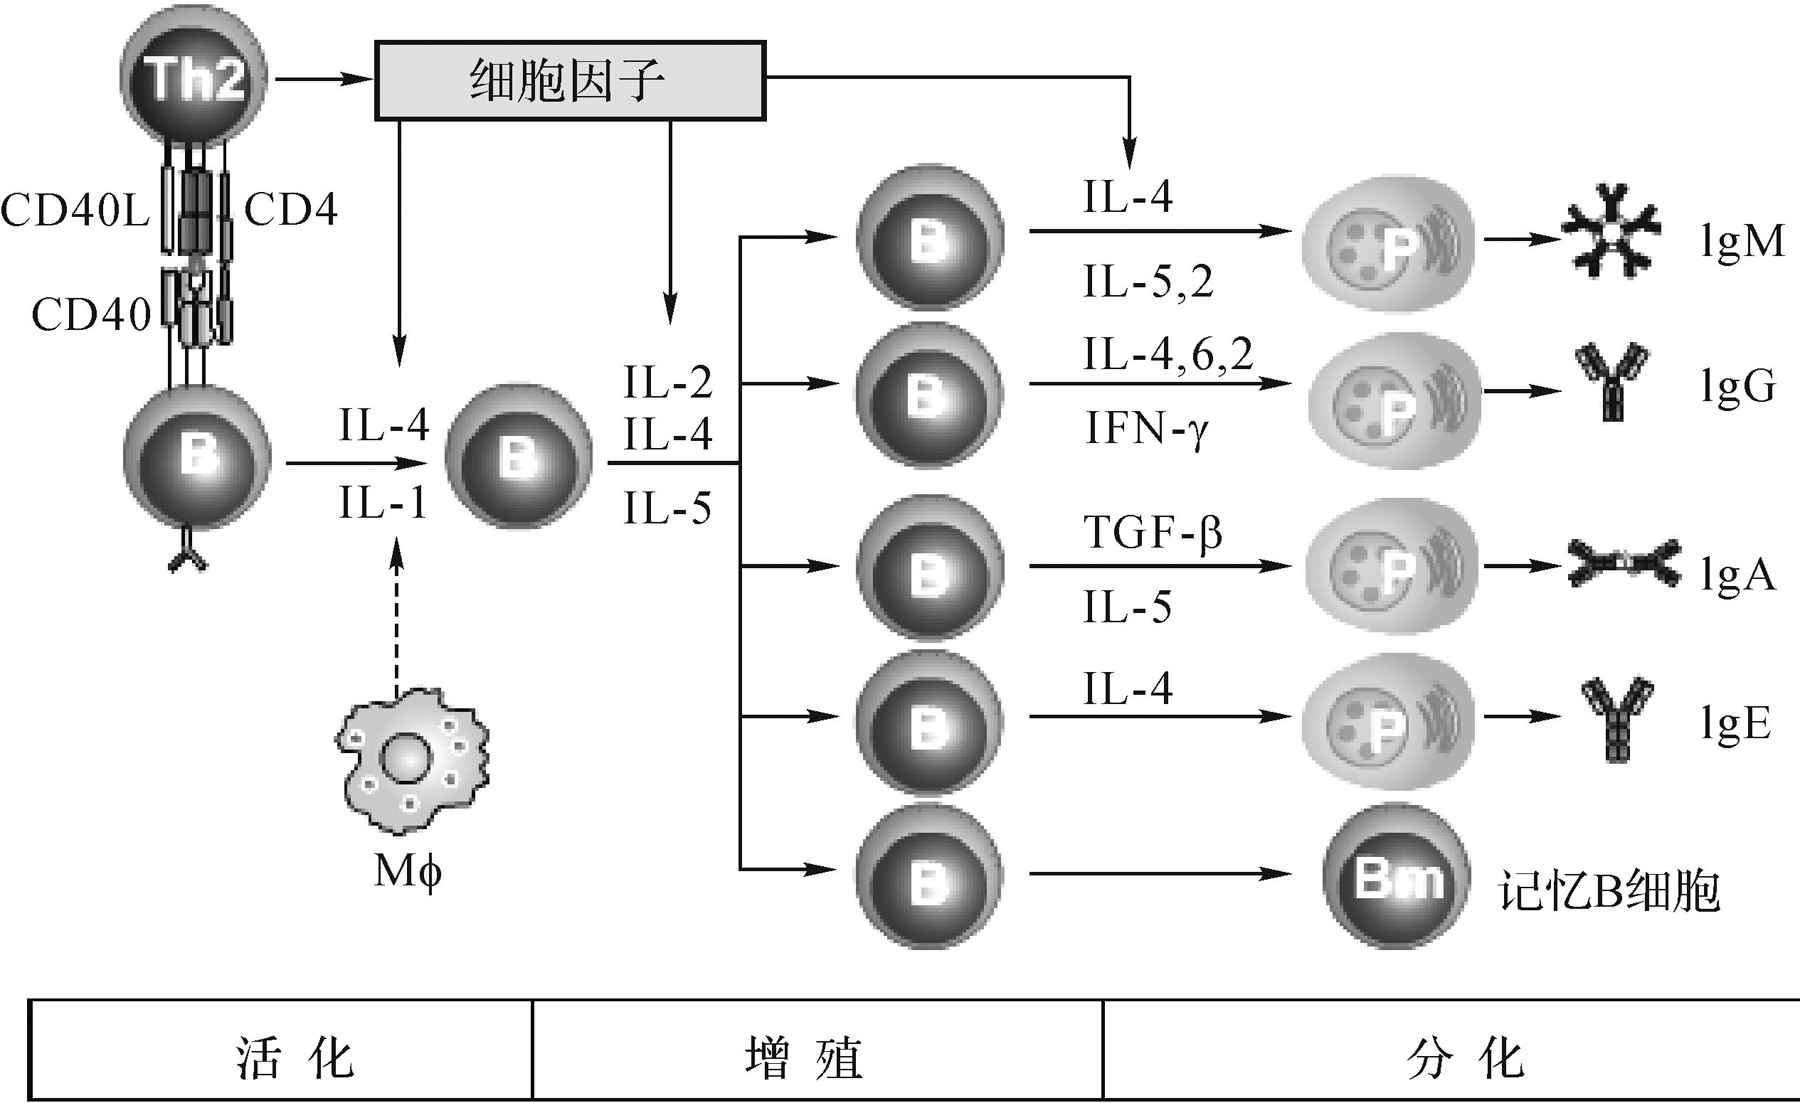
\includegraphics{./images/Image00145.jpg}
 \captionsetup{justification=centering}
 \caption{B细胞活化过程示意图}
 \label{fig9-19}
  \end{figure} 


\subsection{抗体产生的一般规律}

病原体初次侵入机体所引发的应答称为初次免疫应答(primary immune
response)。在初次应答的晚期,随着抗原被清除,多数效应T细胞和浆细胞均发生死亡,同时抗体浓度逐渐下降(图\ref{fig9-20})。但是,应答过程中所形成的记忆性T细胞和B细胞具有长寿命而得以保存,一旦再次遭遇相同抗原刺激,记忆性淋巴细胞可迅速、高效、特异地产生应答,此即再次免疫应答(secondary
response)。

\begin{figure}[!htbp]
 \centering
 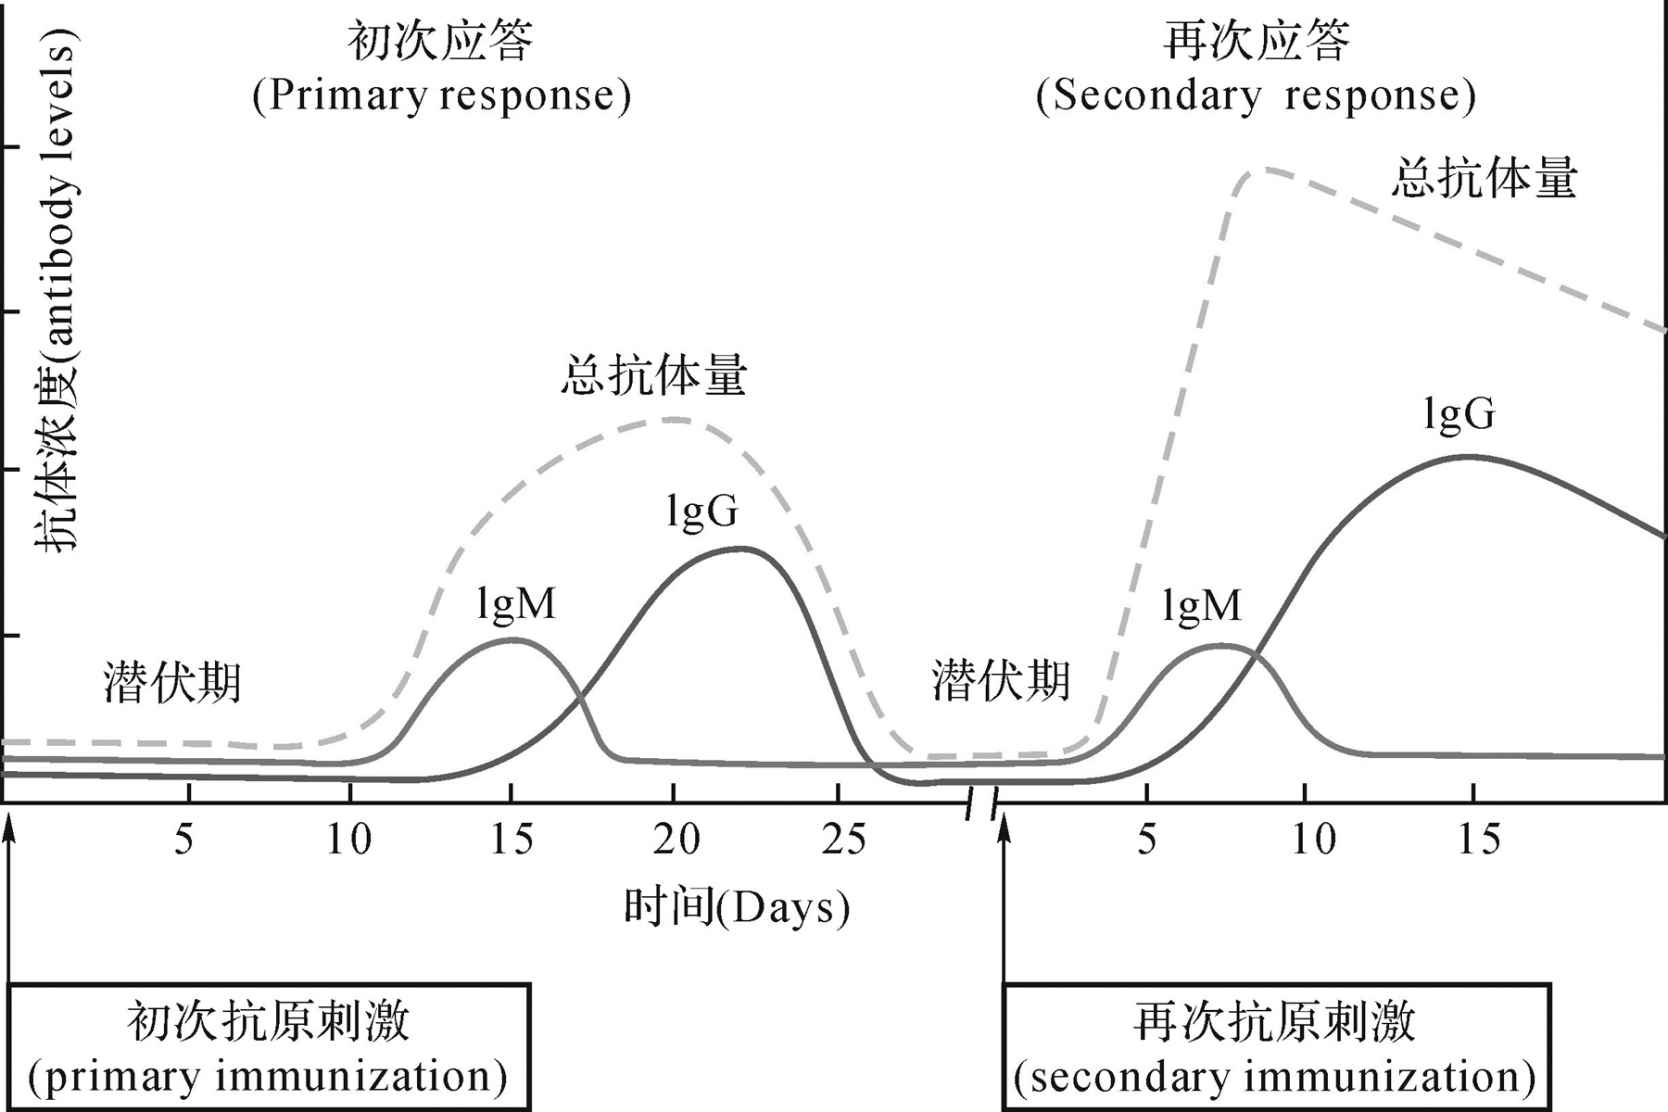
\includegraphics{./images/Image00146.jpg}
 \captionsetup{justification=centering}
 \caption{抗体产生的一般规律}
 \label{fig9-20}
  \end{figure} 

(一)初次应答

机体初次接受适量Ag
免疫后,需经一定的潜伏期,才能在血清中出现Ab,该种Ab含量低,持续时间短,这种现象称为初次应答。TDAg
以IgM 为主,IgG出现较晚。

(二)再次应答

同一抗原再次侵入机体,免疫系统可迅速、高效地产生特异性应答。由于记忆性B细胞表达高亲和力BCR,可竞争性结合低剂量抗原而被激活,故仅需很低抗原量即可有效启动再次免疫应答。再次应答过程中,记忆性B细胞作为APC摄取、处理抗原,并将抗原递呈给记忆性Th细胞。激活的Th细胞所表达的多种膜分子和大量分泌型细胞因子又作用于记忆性B细胞,使之迅速增殖并分化为浆细胞,合成和分泌Ab,Ab含量大幅度上升,且维持时间长久,这种现象称为再次应答。

特点:(1)潜伏期明显缩短,(2)产生高水平Ab,(3)Ab绝大部分为IgG。IgM与初次应答相似。

表\ref{tab9-1}中归纳出初次与再次免疫应答特性比较。

\begin{longtable}[]{@{}lll@{}}
    \caption{初次与再次免疫应答特性比较}
    \label{tab9-1}\\
\toprule
特性 & 初次 & 再次\tabularnewline
\midrule
\endhead
抗原递呈 & 非B 细胞 & B 细胞\tabularnewline
抗原浓度 & 高 & 高\tabularnewline
延迟相 & 5 ~ 10 天 & 2 ~ 5 天\tabularnewline
Ig 类别 & 主要为IgM & IgG 、IgA 等\tabularnewline
亲和力 & 低 & 高\tabularnewline
无关抗体 & 多 & 少\tabularnewline
\bottomrule
\end{longtable}


\subsection{B细胞应答的效应}

B细胞应答的主要效应分子为特异性抗体,它可通过多种机制发挥免疫效应,以清除非己抗原(图\ref{fig9-21})。

1.中和作用:中和毒素和病原体,阻止其入侵宿主细胞。

2.免疫调理作用:IgG、IgA抗体借助其Fab段与病原体结合,借助其Fc段与吞噬细胞表面FcR结合,从而促进吞噬细胞吞噬病原体,此效应即抗体介导的调理作用。

3.激活补体:IgG和IgM类抗体与抗原结合形成免疫复合物,可通过经典途径激活补体系统,从而发挥补体介导的杀菌、溶菌作用。另外,补体激活所产生的C3b结合在病原体表面,可与吞噬细胞表面C3bR结合,从而促进吞噬细胞吞噬病原体,此为补体介导的调理作用。

4.抗体依赖性细胞介导的细胞毒作用(ADCC):抗体IgG的Fab段与抗原结合,Fc段与NK细胞、巨噬细胞、中性粒细胞和嗜酸粒细胞的FcγRIII结合,介导效应细胞杀伤携带特异性抗原的靶细胞,此为ADCC作用。

5.分泌型IgA的局部抗感染作用:分泌型IgA分泌至呼吸道、消化道和生殖道黏膜表面,可阻止细菌、病毒和其他病原体入侵。

6.免疫损伤作用:

(1)超敏反应与自身免疫病:由抗体引起的免疫损伤可见于I、II、III型超敏反应和自身免疫病。I型超敏反应由IgE介导,II、III型超敏反应由IgG、IgM介导。某些自身免疫病损伤与II、III型超敏反应有关。

(2)移植排斥反应:受者体内存在针对移植物抗原的预存抗体(IgG),可导致超急性排斥反应。另外,体液免疫应答在急、慢性排斥反应中也有一定作用。

(3)促进肿瘤生长:肿瘤患者产生的某些IgG亚类可作为封闭因子,阻碍特异性CTL识别和杀伤肿瘤细胞,从而促进肿瘤生长。

\begin{figure}[!htbp]
 \centering
 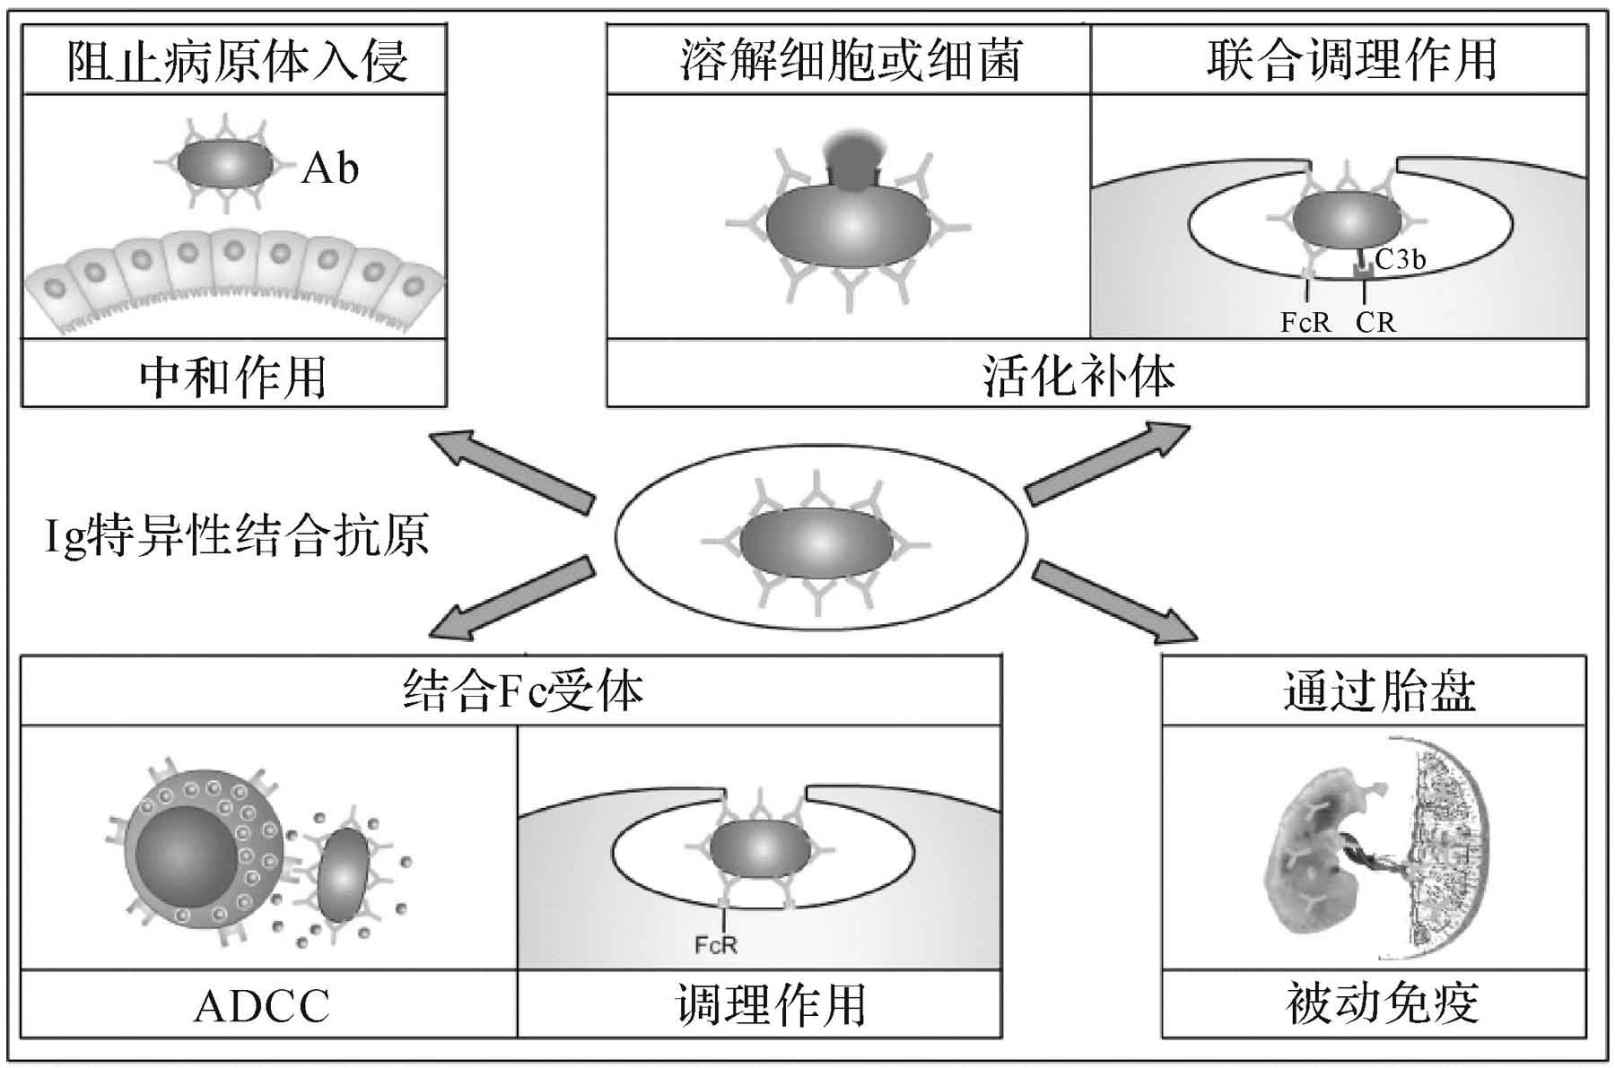
\includegraphics[width=.6\textwidth]{./images/Image00147.jpg}
 \captionsetup{justification=centering}
 \caption{B细胞应答的效应}
 \label{fig9-21}
  \end{figure} 

\section{T细胞介导的细胞免疫应答}

T细胞介导的细胞免疫应答通常由TDAg引起,在多种免疫细胞和CK协同作用下完成(图\ref{fig9-22}),其中免疫细胞包括:①APC:如MM、树突状细胞,病毒感染的靶细胞。②CD4\textsuperscript{+}
TH 细胞:具有免疫调节作用。③效应T细胞:CD4\textsuperscript{+}
Th1、CD8\textsuperscript{+} T细胞(CTL)。

\begin{figure}[!htbp]
 \centering
 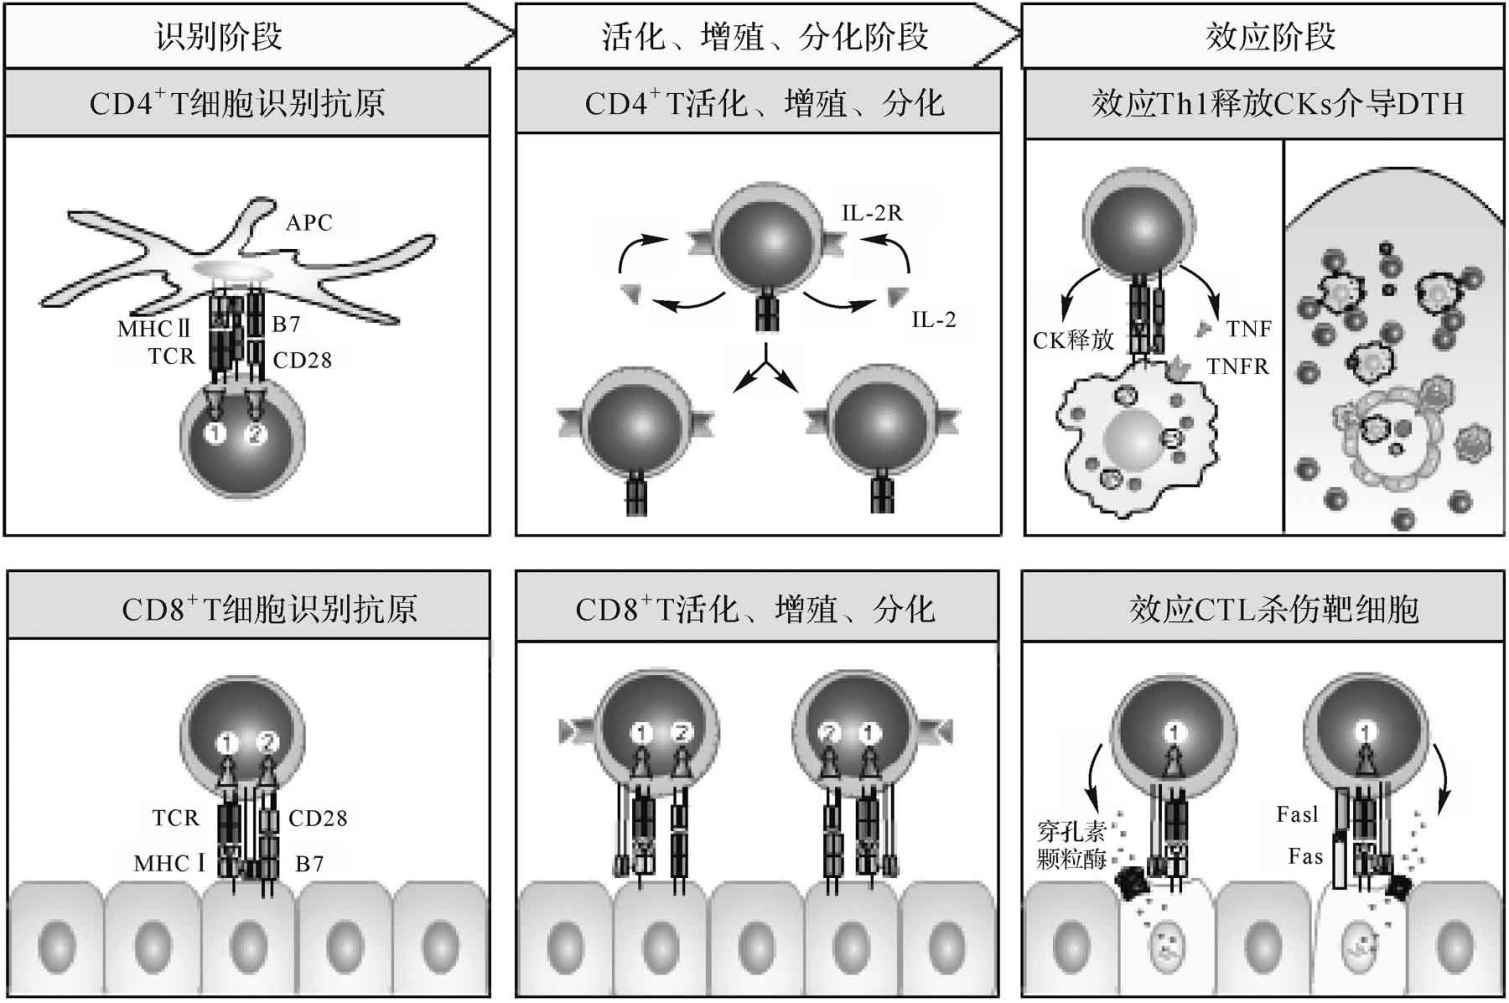
\includegraphics[width=.66\textwidth]{./images/Image00148.jpg}
 \captionsetup{justification=centering}
 \caption{细胞免疫应答的基本过程}
 \label{fig9-22}
  \end{figure} 


\subsection{效应T细胞的生物学特征}

由初始T细胞增殖、分化而来的效应T细胞具有如下特征:

1.合成并分泌多种效应分子:效应T细胞可分泌多种活性分子,如细胞毒素(穿孔素、颗粒酶等)、各种蛋白酶、细胞因子等。

2.膜分子表达及生物学活性发生明显改变:效应T细胞表达的膜分子不同于初始T细胞,并表现出生物学活性的明显改变。例如:高表达FasL可介导靶细胞凋亡;表达整合素(如VLA-4)可促使效应T细胞与炎症部位血管内皮细胞黏附,有助于效应T细胞向感染部位浸润并发挥效应;高表达CD2和LFA-1可增强T细胞与靶细胞结合的亲和力。


\subsection{CTL介导的细胞毒效应}

CTL主要杀伤胞内寄生病原体(病毒、某些胞内寄生菌等)的宿主细胞、肿瘤细胞等。CTL多为CD8\textsuperscript{+}
T细胞,可识别MHC-I类分子递呈的抗原;约10\%的CTL为CD4\textsuperscript{+}
T细胞,可识别MHC-Ⅱ类分子递呈的抗原。CTL可高效、特异性地杀伤靶细胞,而不损害正常组织。

1.效-靶细胞结合:CD8\textsuperscript{+}
T细胞在外周淋巴组织内增殖、分化为效应CTL,在趋化因子作用下离开淋巴组织向感染灶集聚。

效应CTL高表达黏附分子(如LFA-1、CD2等),可有效结合表达相应受体(ICAM、LFS-3等)的靶细胞。一旦TCR遭遇特异性抗原,TCR的激活信号可增强效-靶细胞表面黏附分子对的亲和力,并在细胞接触部位形成紧密、狭小的空间,使CTL分泌的非特异性效应分子集中于此,从而选择性杀伤所接触的靶细胞,但不影响邻近正常细胞。

2.CTL的极化(polarization):CTL的TCR与靶细胞表面肽-MHC-I类分子复合物特异性结合后,TCR及共受体向效-靶细胞接触部位聚集,导致CTL内亚显微结构极化,即细胞骨架系统(如肌动蛋白、微管)、高尔基复合体及胞浆颗粒等均向效-靶细胞接触部位重新排列和分布,从而保证CTL分泌的非特异性效应分子选择性作用于所接触的靶细胞。

3.致死性攻击:CTL主要通过两条途径杀伤靶细胞(图\ref{fig9-23})。

\begin{figure}[!htbp]
 \centering
 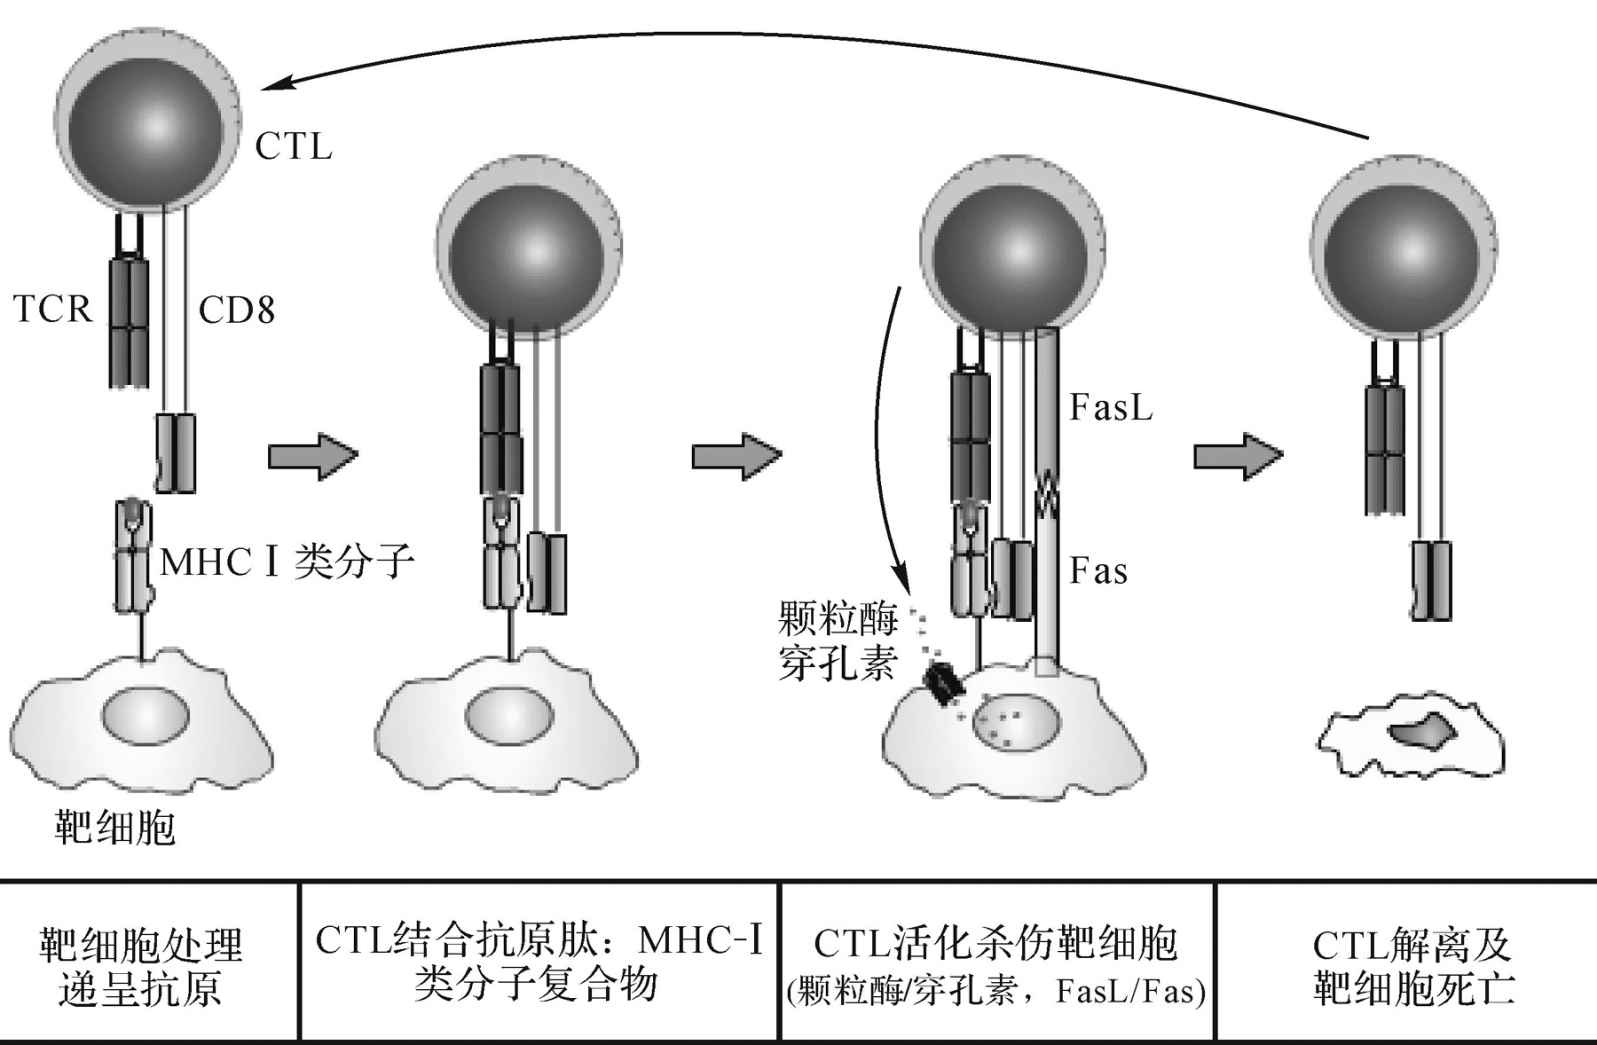
\includegraphics[width=.6\textwidth]{./images/Image00149.jpg}
 \captionsetup{justification=centering}
 \caption{CTL杀伤靶细胞的过程}
 \label{fig9-23}
  \end{figure} 

(1)穿孔素/颗粒酶途径:穿孔素(perforin)是储存于胞浆颗粒中的细胞毒素,其生物学效应类似于补体激活所形成的膜攻击复合体(MAC)。穿孔素单体可插入靶细胞膜,在钙离子存在的情况下,聚合成内径为16nm的孔道,使水、电解质迅速进入细胞,导致靶细胞崩解。

颗粒酶(granzyme)也是一类重要的细胞毒素,属丝氨酸蛋白酶。颗粒酶随CTL脱颗粒而出胞,循穿孔素在靶细胞膜所形成的孔道进入靶细胞,通过激活凋亡相关的酶系统而介导靶细胞凋亡。

(2)TNF与FasL途径:效应CTL可分泌TNF-α、TNF-β并表达膜FasL。这些效应分子可分别与靶细胞表面TNFR和Fas结合,通过激活胞内Caspase系统,介导靶细胞凋亡。

CTL的胞毒效应主要介导靶细胞凋亡,其生物学意义为:在清除感染细胞时,无细胞内容物(如溶酶体酶等)的外漏,可保护正常组织细胞免遭损伤;靶细胞凋亡过程中激活内源性核苷酸内切酶,可降解病毒DNA,从而阻止细胞死亡所释放的病毒再度感染旁邻正常组织细胞。

效应CTL杀死靶细胞后即与之脱离,并可再次与表达相同特异性抗原的靶细胞结合,对其发动攻击,从而高效、连续、特异性地杀伤靶细胞。


\subsection{Th1细胞介导的细胞免疫效应}

某些胞内寄生的病原体(如分支杆菌属的结核杆菌和麻风杆菌)可在巨噬细胞的吞噬小体内生长,并逃避特异性抗体和CTL攻击。针对此类胞内寄生病原体,Th1细胞可通过活化巨噬细胞及释放各种活性因子而攻击之(图\ref{fig9-24})。

\begin{figure}[!htbp]
 \centering
 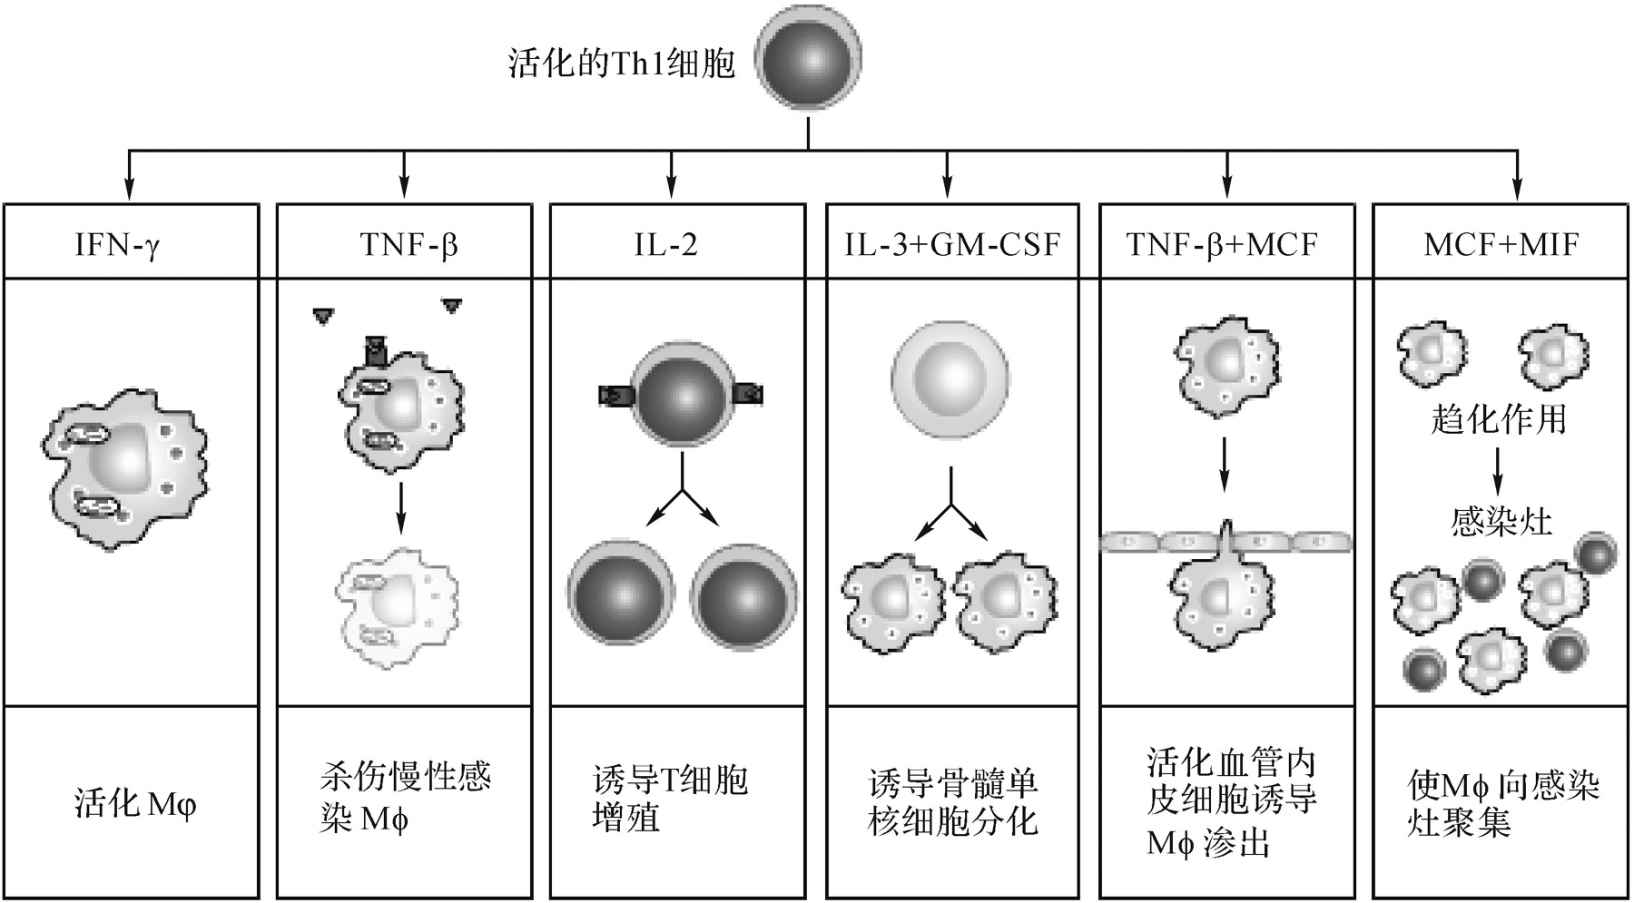
\includegraphics[width=.6\textwidth]{./images/Image00150.jpg}
 \captionsetup{justification=centering}
 \caption{Th1细胞在抗胞内病原体感染中的作用}
 \label{fig9-24}
  \end{figure} 

1.Th1细胞对巨噬细胞的作用:Th1细胞可产生多种细胞因子,通过多途径作用于巨噬细胞。

(1)激活巨噬细胞:Th1细胞与巨噬细胞所递呈的特异性抗原结合,可诱导巨噬细胞激活,其机制为:Th1细胞诱生IFN-γ等巨噬细胞活化信号;Th1细胞表面CD40L与巨噬细胞表面CD40结合,可向巨噬细胞提供敏感信号,从而有效激活之。

活化的巨噬细胞通过不同机制杀伤胞内寄生的病原体,例如:产生NO和超氧离子;促进溶酶体与吞噬体融合;合成并释放各种抗菌肽和蛋白酶,等等。

另一方面,活化的巨噬细胞也可进一步增强Th1细胞的效应,其机制为:①激活的巨噬细胞高表达B7和MHC-Ⅱ类分子,从而具有更强的递呈抗原和激活CD4\textsuperscript{+}
T细胞的能力;②激活的巨噬细胞分泌IL-12,可促进Th0细胞向Th1细胞分化,进一步扩大Th1细胞应答的效应。

(2)诱生并募集巨噬细胞:其机制为 ①
Th1细胞产生IL-3和GM-CSF,促进骨髓造血干细胞分化为巨噬细胞;②Th1细胞产生TNF-α、TNF-β和MCP-1等,可分别诱导血管内皮细胞高表达黏附分子,促进巨噬细胞和淋巴细胞黏附于血管内皮,继而穿越血管壁,并通过趋化运动被募集至感染灶。

2.Th1细胞对T细胞的作用:Th1细胞产生IL-2等细胞因子,可促进Th1细胞、CTL等增殖,从而放大免疫效应。

3.Th1细胞对B细胞的作用:Th1细胞也具有辅助B细胞的作用,促使其产生具有强调理作用的抗体,从而进一步增强巨噬细胞对病原体的吞噬。

4.Th1细胞对中性粒细胞的作用:Th1细胞产生淋巴毒素和TNF-α,可活化中性粒细胞,促进其杀伤病原体的作用。


\subsection{细胞免疫应答生物学效应}

1.抗胞内寄生性病原体感染;

2.抗肿瘤免疫;

3.免疫损伤(某些自身免疫病、药物过敏反应和迟发型超敏反应);

4.参与同种移植排斥反应和介导移植物抗宿主反应。

\noindent\textbf{【理解与思考】}

1.如果你是一个单核巨噬细胞,当你发现病原微生物入侵时,会产生哪些生物学作用?

2.当一个正常的细胞发生癌变时,它即将遭遇什么?你能形象地叙述一下吗?

3.结合第二章免疫系统中的淋巴细胞的产生,你能描绘出淋巴细胞短短的一生,从产生、经历及结局吗?

4.结合免疫应答的整个过程,请分别给诸如造血干细胞、淋巴细胞、树突状细胞、单核-巨噬细胞、粒细胞、肥大细胞、红细胞等各种免疫细胞在体内的作用加以定位。

5.如果你是一位医生,你的病人在器官移植后,病人体内可能发生什么变化?你要采取哪些措施保证移植器官存活?

\noindent\textbf{【课外拓展】}

1.树突状细胞还有哪些种类?各有何特点及生物学作用?

2.细胞死亡或凋亡后,形态结构有何变化?

3.影响抗体类别转换的因素有哪些?

\noindent\textbf{【课程实验与研究】}

1.请设计检测某一种免疫细胞的活性的路线图。

2.如何证明诸如蜂皇浆等能促进免疫细胞生成和活性的特性?

3.美国加利福尼亚大学洛杉矶分校以及乔治•梅森大学的研究人员共同完成接种天花疫苗或可预防艾滋病的研究,如果你是其中的一员,请设计一实验路线图。

\noindent\textbf{【课程研讨】}

1.针对细菌、胞内病原微生物、癌变细胞,机体的免疫应答有何不同?为什么?

2.免疫细胞膜分子MHC-I类、MHC-II类的分布与免疫应答有何关系?为何有的肿瘤细胞会产生免疫逃逸?

3.一个自身的组织细胞,是否有可能遭遇免疫清除?为什么?

\noindent\textbf{【课后思考】}

1.单核吞噬细胞系统、树突状细胞、B细胞生物学特性是什么?

2.免疫应答包括哪些基本过程?

3.抗体的初次应答与再次应答各有何特点?

4.T、B细胞介导的免疫应答各有何特点?

\noindent\textbf{【课外阅读】}

\begin{center}
 \textbf{\Large HIV-1感染的T细胞免疫应答}
 \end{center}

HIV-1感染可以同时活化T细胞免疫与体液免疫。所活化的免疫反应尽管对病毒有一定的抑制作用,但不能清除病毒,因而,HIV-1感染均形成慢性持续性感染,最后大部分个体以免疫系统功能耗竭、严重的免疫缺陷为结局,感染者可因病发感染或肿瘤而死亡。大量的研究表明,HIV-1特异性T细胞在与HIV做斗争中起极其重要的作用。

\begin{center}
 {\large 一、T细胞的作用}
 \end{center}

HIV-1特异性CD8\textsuperscript{+}
T细胞可利用穿孔素和颗粒酶B或CD95L直接杀伤被HIV-1感染的细胞,从而消除感染原;也可产生细胞因子(比如IFN-γ)来抑制病毒的复制;或者释放趋化因子(比如MIP-1α、MIP-1β和RANTES)来阻断病毒进入新的靶细胞。控制HIV-1病毒复制的能力依赖于结构与功能健全的HIV-1特异性CD8\textsuperscript{+}
T细胞。许多HIV-1感染病人的CD8\textsuperscript{+}
T细胞上的CD3链和CD28受体有缺陷,或者CD8\textsuperscript{+}
T细胞合成细胞毒性分子(如穿孔素)与细胞因子(干扰素)有缺陷。这些缺陷可导致CD8\textsuperscript{+}
T细胞的功能受到损伤时,病人体内即使可检测到活跃的HIV-1特异性CD8\textsuperscript{+}
T细胞,病人依然不能有效控制病毒。另外,研究表明,HIV-1特异性CD8\textsuperscript{+}
T细胞识别表位区的突变可以导致病毒载量的急剧上升以及病情向AIDS期恶化。

HIV病毒破坏CD4\textsuperscript{+}
T淋巴细胞,当期数量下降到200个/uL以下时,就被诊断为患有艾滋病并且需要接受抗逆转录治疗。由于HIV-1可优先感染HIV-1特异性CD4\textsuperscript{+}
T细胞,随着病情的进展,HIV-1特异性CD4\textsuperscript{+}
T细胞会逐渐减少乃至完全耗竭。HIV-1特异性CD4\textsuperscript{+}
T细胞的主要功能在于维护HIV-1特异性CD8\textsuperscript{+}
T细胞上,而不是在直接抗击HIV-1中。以前的研究表明,CD4\textsuperscript{+}
T细胞在CD8\textsuperscript{+}
T细胞免疫反应的激活、记忆性CD8\textsuperscript{+}
T细胞的功能成熟等过程中起重要的作用。相应地,HIV-1感染导致CD4\textsuperscript{+}
T细胞的耗竭,可导致HIV特异性的记忆CD8\textsuperscript{+}
T细胞的成熟障碍,以及HIV-1特异性CD8\textsuperscript{+}
T细胞的功能受损。由于CD4\textsuperscript{+}
T细胞与B细胞间的相互作用对B细胞的分化成熟及其后抗体的产生极为重要,因而在HIV感染晚期,随着CD4\textsuperscript{+}
T细胞的缺失,感染者产生新的中和抗体的能力逐渐降低。

总之,HIV-1特异性的CD8\textsuperscript{+}
T细胞在直接抗击HIV-1中起主导作用,CD4\textsuperscript{+}
T细胞主要是辅助CD8\textsuperscript{+}
T细胞和B细胞。所以,有效的抗艾滋病疫苗应该能同时活化HIV-1特异性CD4\textsuperscript{+}
T细胞与CD8\textsuperscript{+} T细胞。

\begin{center}
 {\large 二、HIV-1的免疫逃逸}
 \end{center}

HIV-1感染后可同时活化T细胞免疫和体液免疫,逃逸免疫系统的攻击成为HIV-1生存的重要内容。

HIV-1逃逸机制主要包括:通过Nef蛋白下调I类HLA分子表达,从而降低病毒抗原的递呈;通过损伤T
细胞的功能,降低T
细胞的攻击能力;通过T细胞识别表位内的点突变,降低病毒表位与HLA分子的结合能力或完全取消结合,或者突变能够与T细胞受体结合并抑制T细胞功能的肽序列;也可以通过表位旁序列的突变使得机体的蛋白酶不能切割形成表位序列。尽管以上各种机制并存,但通过突变T细胞的免疫攻击仍然是病毒应用的最主要机制。

事实上,HIV感染后,突变性逃逸不断地发生并贯穿病毒的整个感染过程。病毒逃逸不同的表位特异性T细胞所需要的时间是不同的。在HIV-1感染者中发现,虽然B57限制性的GagTW10表位特异性CD8\textsuperscript{+}
T细胞与B27限制性的GagKK10表位特异性CD8\textsuperscript{+}
T细胞同样具有保护作用,且均在感染早期被激活,但病毒对前者的逃逸在感染早期就可以发生,而对于后者的逃逸通常发生在感染晚期。HIV-1病毒的逃逸一般来说是有代价的,代价的大小决定于CD8\textsuperscript{+}
T细胞免疫反应所攻击部位对病毒生存的重要性。针对HIV-1Gag的免疫反应对病毒造成的损伤较大,因而病毒难以逃脱。在B27限制性的GagKK10表位的逃逸中,主要的逃逸突变R264K(这一突变可导致表位不能与B27结合)可能发生在病毒载量升高之前,因为这一逃逸株并不能生存,而只有等到另外一个补偿性突变L268M发生时,病毒载量才可能升高,也就是说,在没有补偿性突变发生前,逃逸性突变对病毒是致命的。并不是每一个逃逸突变都需要病毒付出重大的代价。在HIV-1感染的人群中,大部分表位的逃逸突变对病毒伤害不大,从而在病毒的传播中获得保留。这样从整个HIV-1感染的群体考虑,对病毒抑制起显著作用的表位因很快地回复突变而在群体中保留下来,从而成为病毒序列中保守的序列;反之,在群体中显示多样性的序列对病毒的生存可能并不产生重要影响。有效的HIV疫苗应该能够有效活化针对病毒保守区免疫反应,我国科学家在国际上首次提出并尝试了一个新的疫苗策略,这一策略可以实现优先活化针对病毒保守区的免疫反应。

\begin{center}
 {\large 三、HIV感染后不同时期,T细胞免疫应答特征}
 \end{center}

从上面的叙述可知,HIV-1感染后的T细胞免疫应答在不同感染时期的特征有很大差异。

(一)感染早期

1.至少在感染之后10天内,机体外周血中检测不到明显的T细胞应答,病毒在这段时间内大量扩增,在不同的靶细胞中形成潜伏库,为病毒长期持续性感染奠定基础;

2.感染10天后(2~3周),随着病毒的进一步扩增,产生大量的T细胞免疫反应,病毒载量随着CD8\textsuperscript{+}
T细胞免疫反应的出现与升高开始下降,并逐步到达一个稳定点,这种病毒载量与HIV-1特异性CD8\textsuperscript{+}
T细胞免疫反应的逆向互动被认为是由于CD8\textsuperscript{+}
T细胞对病毒抑制所致;

3.活化的T细胞免疫应答以针对病毒的优势表位为主,免疫反应狭窄,其中以针对Nef与Gag的免疫反应为主;

4.病毒感染时,免疫系统依然健康,因而感染早期活化的HIV-1特异性T细胞具有多种功能,包括IL-2分泌功能与增殖功能,对病毒的抑制能力较强;

5.在感染早期,T细胞免疫反应越高,对病毒抑制越强,病程进展就越缓慢,预后就越好;

6.由于病毒的大量扩增,而HIV-1特异性CD4\textsuperscript{+}
T细胞被优先感染,因而,这一时期对HIV-1特异性CD4\textsuperscript{+}
T细胞的消耗严重;病毒载量越高,CD4\textsuperscript{+}
T细胞的损耗越重,病程进展也越快,预后越差;

7.在这一阶段内,免疫逃逸已经大量发生,逃逸株已经出现,逃逸的后果各不相同。

(二)感染进入慢性期

如果病毒复制得不到控制,随着感染的持续,免疫反应出现一些新的特征:

1.由于针对免疫优势表位的逃逸持续发生,越来越多的亚优势表位被免疫系统识别,因而免疫反应识别的表位越来越多,免疫反应更为广泛。

2.新活化的、针对亚优势表位的T细胞免疫反应引发,由于缺乏足够的CD4\textsuperscript{+}
T细胞辅助,功能上可存在缺陷。

3.由于免疫系统处于持续性的高度激活状态,T细胞处于大量扩展及随后的大量凋亡的循环更替中,这种状态的持续导致记忆性细胞库耗竭,只是体内以效应型T细胞为主。

4.HIV-1特异性T细胞出现功能损伤,表现为细胞病毒性分子的合成障碍、IL-2分泌性细胞减少、增殖能力下降甚至完全丧失增殖能力。

5.由于T细胞功能受损,抑制病毒能力下降甚至丧失,因而,这一时期可表现为HIV-1特异性T细胞随着病毒载量的升高而升高,但T细胞的升高却不能抑制病毒的复制,不能降低病毒载量。

6.针对病毒Gag保守区的免疫反应依然与病毒载量呈现负相关。

如果在感染早期机体能够控制病毒复制,那么,尽管机体不能清除病毒,但个体的疾病进展将非常缓慢,常成为长期不进展者,此时体内的T细胞免疫应答特征与感染早期的特征相似。

\begin{center}
 {\large 四、人体对HIV-2病毒的免疫应答有助于艾滋病疫苗研发}
 \end{center}

科学家发现,感染2型人类免疫缺陷病毒(HIV-2)但是不发病的人们能针对一种特定的病毒蛋白质产生很强的免疫应答。这项研究可能有助于开发艾滋病疫苗。

HIV-2与HIV-1不同,前者很少造成艾滋病发病,大约80\%的HIV-2患者从不表现出临床症状。来自冈比亚共和国、几内亚比绍共和国和英国的科学家分析了来自几内亚比绍的一组共64名无症状的HIV-2患者。
他们发现这些患者的免疫系统------特别是他们的一种免疫细胞T细胞------能够对一种名为Gag的病毒蛋白质做出显著的反应,这帮助了他们控制病毒的复制。Gag也是HIV-1病毒的成分。人体对Gag蛋白的反应越强,血液中的HIV-2病毒的水平就越低。那些反应最强的患者的血液中检测不到病毒。

证明了在HIV-2患者中,T细胞的免疫应答足够控制感染。这一发现很重要,因为科学家在设计疫苗的时候,必须决定应该激活哪种免疫系统(抗体还是T细胞),用于对抗HIV。
HIV患者产生针对Gag蛋白的T细胞用于控制病毒复制,知道这一事实可以开发基于T细胞的预防和治疗性疫苗。这是科学家首次研究无症状的HIV-2患者,这可以让科学家分析他们的保护性的免疫应答。一些无症状的HIV-1患者也对这种蛋白产生了很强的免疫应答。

\begin{center}
 \textbf{\Large 免疫细胞CD\textsuperscript{+} \textsubscript{8}T淋巴细胞帮助控制艾滋病毒}
 \end{center}


有些人对艾滋病有一种天生的免疫能力,他们能够控制艾滋病病毒侵入自己身体,医学专家发现他们体内有一种免疫细胞CD$_8^+$
T淋巴细胞,而且这种细胞的作用方式使人具有特别强的免疫能力。这一新的医学突破为艾滋病的防治指明了方向。

这项新的研究发表在权威杂志《免疫》(Immunity)上,分析了一些对艾滋病具有免疫能力的人的体内机制,解释了他们为什么能够控制病毒,以及如何消灭体内受艾滋病感染的细胞。美国马里兰州贝塞斯达的国立卫生研究院免疫学家、艾滋病毒疫苗研究者马克•康诺斯(MarkConnors)说:“这一发现是这一领域的一大突破。”

康诺斯说:“有些人(小于0.5\%)第一次感染艾滋病后几十年都不犯病,因为他们控制了病毒的扩散,同时让病毒死于无形之中。曾经有研究表明这种控制能力与体内的一种免疫细胞------CD$_8^+$
T淋巴细胞有关,这种免疫细胞能发现并消灭被病毒感染的细胞。但当时无法解释究竟为什么会这样。

现在康诺斯和他的研究团队发现有较多CD$_8^+$
T细胞的人通过将毒液输送到受感染的细胞,从而控制艾滋病的发作。为了获得这一发现,科学家们制订了一系列敏感的测试,分析存在的这些T细胞,以及它们消灭感染艾滋病毒的能力。他们发现CD$_8^+$
T细胞在受感染的人身上生长得非常迅速,从而比一般人更能控制艾滋病。

但他们同时还发现不仅仅是CD\textsuperscript{+} \textsubscript{8}
T淋巴细胞数量增多的问题,还与这些细胞的作用方式紧密相关,因为它们能够生长和提供一对特别的分子“穿孔素”和“颗粒酶B”。穿孔素,顾名思义,就是能够在靶细胞膜上穿孔的物质。细胞被穿孔了,颗粒酶B就能够进入并破坏受感染的细胞。

研究结果对长期持有的模式进行了挑战。康诺斯称,以前大家认为,我们的免疫记忆细胞,比如CD$_8^+$
T细胞,它们的作用就像是“一个装满子弹的枪,根据需要选择子弹杀死病毒”。康纳斯认为,在现实中,这些“记忆细胞”需要重新刺激,在反复接触病毒后需要重新刺激才能够保护我们。

美国马里兰州巴尔的摩市约翰霍普金斯大学医学科学家乔尔•布兰森(JoelBlankson)说:“这项研究成果对发展疫苗意义重大,研究成果为我们评估疫苗疗效提供了新的重要的参数。”他虽然并没有参与其中的工作,但又补充说这项研究“也是一个重要的概念证明,因为它表明,只要艾滋病毒特效杀手T淋巴细胞得到正确的刺激,就可以诱导它发挥作用,从而有效地杀死受艾滋病毒感染的细胞”。

这意味着我们未来能够生产出一种对抗艾滋病感染的治疗性疫苗,而不是单纯的保护感染艾滋病的预防性疫苗。

位于美国费城的宾夕法尼亚大学免疫学家乔托(GuidoSilvestri)称,他对这项研究抱有很大希望。“这样的研究可能将最终为以免疫为基础的干预铺平道路,这样可以利用人体免疫系统的方式,完全控制甚至消灭艾滋病毒。当然,我们还有很长的路要走,至少10年到20年。但是我们已经向正确方向迈出了重要的一步。”

康诺斯表示,下一步他们的研究重点将放在为什么大多数人的CD$_8^+$ T细胞缺乏杀死艾滋病毒感染的细胞的能力。

\begin{center}
 \textbf{\Large Immunity:T细胞记忆机制}
 \end{center}

澳大利亚国立大学医学研究所、化学研究所的科学家发现新的免疫理论,相关成果公布在《Immunity》上,并列为封面文章。

众所周知,B细胞具有记忆性。一般来说,B细胞的记忆性的形成与DNA序列的改变有联系,B细胞通过改变DNA序列来维持细胞的记忆性。但是,免疫细胞的记忆性机制研究比较多的是B细胞,相比之下,T细胞研究得比较少。

研究小组发现,记忆性T细胞的分化过程中,RNA重排起重要作用。研究小组以小鼠的研究模型,通过沉默一个记忆性T细胞分化的关键基因ptprc(产生记忆性T细胞CD45RO的重要基因),结果发现记忆性T细胞的比例发生改变。并且RNA结合蛋白hnRNALL发生改变,会导致RNA的识别区域变得不稳定。

研究者发现,hnrpll突变会导致T细胞不在外周淋巴结聚集,但不影响增殖。对这些突变细胞进行外显子检测分析,结果发现记忆性T细胞的mRNA结合过程发生的广泛的改变。并且相同的变化还出现在神经组织中,这可能是引发记忆性T细胞发生变化的原因。

(资料来源:Immunity,19 December 2008
doi:10.1016/j.immuni.2008.11.004)

